\documentclass[11pt,a4paper]{amsart}
\usepackage[T1]{fontenc}
\usepackage[utf8]{inputenc}
\usepackage{lmodern}
\usepackage[margin=28mm]{geometry}
\usepackage{amsmath,amssymb,amsthm,mathtools,mathrsfs}
\usepackage{enumitem,graphicx,longtable,booktabs,array}
\usepackage[expansion=false]{microtype}
\usepackage[hyphens]{url}
\usepackage{flafter,needspace}
\usepackage{xcolor,tikz,tikz-cd}
\usetikzlibrary{arrows.meta,positioning,calc,fit,backgrounds}
\definecolor{linkblue}{RGB}{29,67,112}
\usepackage[colorlinks=true,linkcolor=linkblue,citecolor=linkblue,urlcolor=linkblue,bookmarksnumbered=true]{hyperref}
\hypersetup{pdftitle={The arithmetic category and stable recovery of lattice factors},pdfauthor={OpenAI},pdfsubject={Arithmetic classification of bifinite correspondences and factor endpoints}}
\numberwithin{equation}{section}
\theoremstyle{plain}
\newtheorem{theorem}{Theorem}[section]
\newtheorem{proposition}[theorem]{Proposition}
\newtheorem{lemma}[theorem]{Lemma}
\newtheorem{corollary}[theorem]{Corollary}
\theoremstyle{definition}
\newtheorem{definition}[theorem]{Definition}
\newtheorem{convention}[theorem]{Convention}
\newtheorem{notation}[theorem]{Notation}
\theoremstyle{remark}
\newtheorem{remark}[theorem]{Remark}
\DeclareMathOperator{\Ad}{Ad}
\DeclareMathOperator{\Hom}{Hom}
\DeclareMathOperator{\Comm}{Comm}
\DeclareMathOperator{\Tr}{Tr}
\DeclareMathOperator{\supp}{supp}
\DeclareMathOperator{\rank}{rank}
\DeclareMathOperator{\ran}{ran}
\DeclareMathOperator{\id}{id}
\DeclareMathOperator{\Aut}{Aut}
\DeclareMathOperator{\GL}{GL}
\DeclareMathOperator{\SL}{SL}
\DeclareMathOperator{\SO}{SO}
\DeclareMathOperator{\SU}{SU}
\DeclareMathOperator{\Sp}{Sp}
\DeclareMathOperator{\Sym}{Sym}
\DeclareMathOperator{\diag}{diag}
\DeclareMathOperator{\Lie}{Lie}
\allowdisplaybreaks[2]
\setlength{\emergencystretch}{2em}
\setlist[enumerate]{leftmargin=*,itemsep=3pt,topsep=5pt}
\setlist[itemize]{leftmargin=*,itemsep=3pt,topsep=5pt}
\pdfinfoomitdate=1
\pdftrailerid{}
\pdfsuppressptexinfo=15
\input{glyphtounicode}
\pdfgentounicode=1
\pdfglyphtounicode{parenleftbig}{0028}
\pdfglyphtounicode{parenrightbig}{0029}
\pdfglyphtounicode{parenleftbigg}{0028}
\pdfglyphtounicode{parenrightbigg}{0029}
\pdfglyphtounicode{parenleftBigg}{0028}
\pdfglyphtounicode{parenrightBigg}{0029}
\pdfglyphtounicode{braceleftBig}{007B}
\pdfglyphtounicode{bracerightBig}{007D}
\pdfglyphtounicode{angbracketleftbig}{27E8}
\pdfglyphtounicode{angbracketrightbig}{27E9}
\pdfglyphtounicode{circleplustext}{2A01}
\pdfglyphtounicode{circleplusdisplay}{2A01}
\pdfglyphtounicode{summationtext}{2211}
\pdfglyphtounicode{summationdisplay}{2211}
\pdfglyphtounicode{productdisplay}{220F}
\pdfglyphtounicode{unionsqdisplay}{2A06}
\pdfglyphtounicode{hatwide}{02C6}
\pdfglyphtounicode{tildewide}{02DC}
\NewCommandCopy{\paperoriginalmapsto}{\mapsto}
\NewCommandCopy{\paperoriginallongmapsto}{\longmapsto}
\DeclareRobustCommand{\mapsto}{\mathrel{%
  \pdfliteral direct{/Span << /ActualText <FEFF21A6> >> BDC}%
  \paperoriginalmapsto
  \pdfliteral direct{EMC}}}
\DeclareRobustCommand{\longmapsto}{\mathrel{%
  \pdfliteral direct{/Span << /ActualText <FEFF27FC> >> BDC}%
  \paperoriginallongmapsto
  \pdfliteral direct{EMC}}}
\DeclareMathOperator{\PSL}{PSL}
\DeclareMathOperator{\PSp}{PSp}
\title[Arithmetic category and stable recovery]{The arithmetic category and stable recovery of lattice factors}
\author{OpenAI}
\date{September 23, 2026}
\begin{document}
\raggedbottom
\begin{abstract}
We prove stable canonical recovery for scalar-twisted group factors of ICC
groups commensurable with property-$(T)$ lattices over characteristic-zero
local fields. Every specified stable isomorphism to a scalar-twisted
factor of any countably infinite ICC group recovers the group, the cocycle
up to a normalized cochain, and equal amplification scales, with an
implementing partial isometry in the given matrix corners. We compute the
arithmetic correspondence subcategory for arbitrary countable ICC groups,
including all bounded maps, summands, conjugates, and Connes fusion, and
combine it with the companion's arithmetic exhaustion theorem.
Multiplication also recovers arbitrary finite-index factor neighbors,
with the exact projective condition on the matched cocycle ratio.
\end{abstract}
\maketitle
\tableofcontents
\clearpage
\section{Introduction}\label{sec:introduction}
A group factor is built from the multiplication of a discrete group, but
an isomorphism of factors need not preserve its distinguished group
unitaries. We ask when the group, a scalar twist of its multiplication,
and the given factor isomorphism can all be recovered. For the lattice
class below, we prove this recovery even after amplification and with an
arbitrary ICC comparison group.

Connes proved countability of
the fundamental group of a property-$(T)$ group factor \cite{Connes1980};
his later problems ask whether nonisomorphic ICC property-$(T)$ groups
have nonisomorphic factors, and ask for the fundamental groups of those
factors \cite[Chapter V, Appendix B.$\varepsilon$, Problems 1--2]{Connes1994}.
The stronger stable formulation displayed by Popa asks for recovery of the
given isomorphism up to a character and inner conjugacy, with amplification
scale one \cite[Section 3, Equations (3.2) and (3.2$'$)]{Popa2007}.

The proof uses the more general relation of finite correspondence:
two factors act normally and commute on one Hilbert space, with finite
module dimensions on both sides. We determine these correspondences
through isomorphisms between finite-index subgroups and finite-dimensional
projective representations. The representation records the ratio of the
two scalar cocycles on the matched subgroups. Neither cocycle separately
need have a finite-dimensional realization.

Our algebraic calculation identifies every bounded map, summand, and
composition of these arithmetic models for arbitrary countable ICC groups.
The geometric exhaustion theorem of the companion
\cite[Theorem~1.2]{ArithmeticCompanion} makes the models exhaustive for the
lattice class. Their integral dimensions recover stable isomorphisms;
their compatibility with multiplication also recovers arbitrary
finite-index factor neighbors.

\subsection{The common conventions and lattice class}
\begin{definition}\label{def:class}
Let $\mathscr K$ be the class of countably infinite ICC groups abstractly
commensurable with a lattice in a finite nonempty product
\[
 G=\prod_{i=1}^r G_i,\qquad G_i=\mathbf H_i(k_i)^+.
\]
Here $k_i$ is $\mathbb R$, $\mathbb C$, or a finite extension of
$\mathbb Q_p$; the primes may differ. The algebraic group $\mathbf H_i$ is
connected, adjoint, and absolutely simple over $k_i$. The superscript $+$
denotes the subgroup generated by the $k_i$-points of the unipotent radicals
of proper $k_i$-parabolic subgroups. Each $G_i$ is required to be noncompact
and to have Kazhdan's property $(T)$.

A lattice is discrete and has finite Haar covolume. Abstract
commensurability means an actual isomorphism between finite-index
subgroups. ICC means that every nonidentity conjugacy class is infinite.
No irreducibility, cocompactness, product decomposition, or torsion
hypothesis is imposed on the lattice.
\end{definition}

For example, $\mathrm{SL}_3(\mathbb Z)$ and every finite-index subgroup
belong to $\mathscr K$. Section~\ref{sec:examples} verifies the lattice and
ICC hypotheses for these and other named examples.

Property $(T)$ means that every continuous unitary representation with
almost invariant unit vectors has a nonzero invariant vector. Standard structure and permanence results for this class are recalled in
Section~\ref{sec:setup}; see also \cite{BHV2008}.

All scalar cocycles take values in $\mathbb T$ and are normalized:
\[
 \mu(g,h)\mu(gh,j)=\mu(h,j)\mu(g,hj),\qquad
 \mu(e,g)=\mu(g,e)=1.
\]
The twisted group factor $L_\mu(\Gamma)$ has canonical unitaries $u_g$
with $u_gu_h=\mu(g,h)u_{gh}$ and trace
$\tau(u_g)=\mathbf1_{\{e\}}(g)$. For an ICC group it is a factor; Section~\ref{sec:setup} recalls the
short Fourier argument.

A bifinite $M$--$N$ correspondence is a Hilbert space with commuting normal
unital left $M$ and right $N$ actions and finite von Neumann module
dimensions on both sides. The actions need not be mutual commutants, and
the correspondence need not be irreducible. Every correspondence in this
paper is separable; every factor isomorphism is normal, unital,
complex-linear, and $*$-preserving. For a finite factor $Q$, write
\[
 Q^t=p\bigl(M_n(\mathbb C)\,\overline\otimes\,Q\bigr)p,
 \qquad (\Tr_n\otimes\tau_Q)(p)=t>0.
\]
The matrix trace $\Tr_n$ is unnormalized; the corner itself has its
normalized trace. The fundamental group of $Q$ is
$\mathcal F(Q)=\{t>0:Q^t\cong Q\}$.

\subsection{Stable canonical recovery}
A stable comparison is an isomorphism between positive amplifications of
two factors. The following theorem forces the amplification scales to agree and
determines the given map on its actual matrix corners.

\begin{theorem}[Presentation equivalence and stable canonical recovery]
\label{thm:stable}
Let $\Lambda\in\mathscr K$ and let $\Pi$ be any countably infinite ICC
group. Let $\omega,\nu$ be arbitrary normalized
scalar cocycles on them, and let $t,s>0$. Then
\[
 L_\omega(\Lambda)^t\cong L_\nu(\Pi)^s
\]
if and only if $t=s$ and there are an isomorphism $\delta:\Lambda\to\Pi$
and a normalized cochain $b:\Lambda\to\mathbb T$ such that
\begin{equation}\label{eq:intro-cochain}
 \omega(g,h)=b(g)b(h)b(gh)^{-1}\nu(\delta(g),\delta(h)).
\end{equation}
Every specified isomorphism at unit scale has the form
\[
 \theta(u_g)=w\,b(g)v_{\delta(g)}w^*
\]
for a unitary $w$ in the target.

More explicitly, put $M=L_\omega(\Lambda)$ and $N=L_\nu(\Pi)$, and let
\[
 \theta:pM_n(M)p\longrightarrow qM_m(N)q
\]
be a specified isomorphism, where the unnormalized traces of $p$ and $q$
are $t$ and $s$. Then $t=s$, and one may choose $\delta,b$ as above and
$z\in M_{m,n}(N)$ so that, for the canonical map
$\varphi(u_g)=b(g)v_{\delta(g)}$,
\[
 z^*z=\varphi^{(n)}(p),\qquad zz^*=q,
 \qquad \theta(x)=z\varphi^{(n)}(x)z^*.
\]
Whenever such an isomorphism exists, the recovered comparison group
$\Pi$ belongs to $\mathscr K$. In particular every factor
$L_\omega(\Lambda)$ in this class has trivial
fundamental group.
\end{theorem}

The untwisted specialization answers the stable recovery question for
Definition~\ref{def:class}, with an arbitrary ICC comparison group.
Property~$(T)$ alone does not imply this recovery. \mbox{OpenAI} constructed a countably
infinite family of pairwise nonisomorphic ICC property-$(T)$ groups with
isomorphic group factors \cite[Chapter~4, Theorem~1.2]{OpenAITenAdvances2026}.
Independently and concurrently, Zhou constructed another pair
\cite[Theorem~A]{Zhou2026}.

\subsection{Arbitrary finite-index factor neighbors}
We next allow the second factor to have no given group presentation.
A \emph{finite-index factor neighbor} of $M$ is a factor joined to $M$
by a nonzero bifinite correspondence. The arithmetic data describing such
a neighbor involve finite-index subgroup isomorphisms rather than an
isomorphism of the whole groups.

For a group $A$, a normalized projective unitary representation with
multiplier $\beta$ is a map $\sigma:A\to\mathcal U(V)$ satisfying
$\sigma(a)\sigma(b)=\beta(a,b)\sigma(ab)$ and $\sigma(e)=I$.
We call $\beta$ \emph{finite type} when such a representation exists with
$0<\dim_{\mathbb C}V<\infty$; its image need not be finite. For a
group homomorphism $\delta$, the pullback cocycle is
$\delta^*\omega(a,b)=\omega(\delta(a),\delta(b))$.

\begin{samepage}
\begin{theorem}[All factor endpoints]\label{thm:endpoints}
Let $\Gamma\in\mathscr K$, let $\mu$ be any normalized scalar cocycle on
$\Gamma$, and let $P$ be a $\mathrm{II}_1$ factor with separable predual.
There is a nonzero bifinite $L_\mu(\Gamma)$--$P$ correspondence if and only if
\[
 P\cong L_\omega(\Lambda)^t
\]
for a countably infinite ICC group $\Lambda$, a normalized scalar cocycle
$\omega$ on $\Lambda$, and $t>0$, for which there are finite-index
subgroups $A\leq\Gamma$ and $B\leq\Lambda$, an actual isomorphism
$\delta:A\to B$, and a nonzero finite-dimensional projective unitary
representation of $A$ with multiplier
\[
 \frac{\mu|_{A\times A}}{\delta^*(\omega|_{B\times B})}.
\]
In particular, the reconstructed group $\Lambda$ belongs to $\mathscr K$.
\end{theorem}
\end{samepage}

The unknown factor $P$ is not assumed to have a group presentation or a
preferred basis. Its presentation is recovered from multiplication in a
finite-index extension. If $\mu=1$, finite-index projective induction
recovers the usual finite-type condition on $\omega$. For arbitrary $\mu$
the ratio condition is essential: $P=L_\mu(\Gamma)$ is always an endpoint.

\subsection{The arithmetic correspondence category}
The two recovery theorems use a common classification of correspondences.
We first describe its models and then the finite-dimensional data that
control their maps and summands.

For finite-index subgroups $A\leq\Gamma$ and $B\leq\Lambda$, an
isomorphism $\delta:A\to B$, and a nonzero finite-dimensional projective
unitary representation $\sigma$ satisfying
\begin{equation}\label{eq:intro-multiplier}
 \sigma(a)\sigma(b)
 =\frac{\mu(a,b)}{\omega(\delta(a),\delta(b))}\sigma(ab),
 \qquad \sigma(e)=I,
\end{equation}
define
\begin{equation}\label{eq:intro-model}
 E(A,B,\delta,\sigma)
 =L^2(M)\,\overline\otimes_{L_{\mu|_A}(A)}
       \bigl(V_\sigma\otimes L^2(N)\bigr),
 \qquad M=L_\mu(\Gamma),\quad N=L_\omega(\Lambda).
\end{equation}
The right $N$ action is standard. The left subgroup action on the second
factor is
$u_a(\xi\otimes\eta)=\sigma(a)\xi\otimes v_{\delta(a)}\eta$.
Equation~\eqref{eq:intro-multiplier} makes this an action with multiplier
$\mu|_A$.


A right action is represented by $\rho(h)\xi=\xi v_h^*$, so
$\rho(h)\rho(k)=\overline{\omega(h,k)}\rho(hk)$.
The left action is $\pi(g)\xi=u_g\xi$. Together they give the joint
action $U_{(g,h)}\xi=u_g\xi v_h^*$.


A \emph{virtual-isomorphism germ} from $\Gamma$ to $\Lambda$ is an
isomorphism between finite-index subgroups, modulo agreement on a common
finite-index subgroup. The action of $\Gamma\times\Lambda$ on germs is
\[
 (g,h)\cdot[\delta]
   =[\Ad(h)\circ\delta\circ\Ad(g^{-1})].
\]
For a germ $d$ let $C_d$ denote its full stabilizer. ICC implies that $C_d$
is the graph of an isomorphism $A_d\to B_d$ between finite-index subgroups;
the proof is included in Section~\ref{sec:calculus}. Use the joint
multiplier
\begin{equation}\label{eq:intro-joint}
 \alpha\bigl((g,h),(g',h')\bigr)
 =\mu(g,g')\overline{\omega(h,h')}.
\end{equation}
For a finite-dimensional $\alpha|_{C_d}$-projective representation
$\sigma_d$, define
\[
 H(d,\sigma_d)=E(A_d,B_d,\delta_d,\widetilde\sigma_d),
 \qquad \widetilde\sigma_d(a)=\sigma_d(a,\delta_d(a)).
\]
Here $\delta_d:A_d\to B_d$ is the isomorphism whose graph is $C_d$.
Section~\ref{sec:calculus} realizes $H(d,\sigma_d)$ as the orthogonal
sum of copies of the representation space indexed by
$(\Gamma\times\Lambda)/C_d$, and describes the induced transports
between them.

The full stabilizer matters because a graph presentation can split one
of these fibres into several pieces. If
$C_\delta=\{(a,\delta(a)):a\in A\}$ represents $d$, the finite set
$C_d/C_\delta$ indexes the pieces that must be grouped together.
Their projective representation is induced from $C_\delta$ to $C_d$
with multiplier $\alpha$. Bimodule projections may mix these pieces;
they become fibre projections only after this grouping.

\Needspace{6\baselineskip}
\begin{theorem}[All finite correspondences]\label{thm:correspondences}
Let $\Gamma\in\mathscr K$, let $\Lambda$ be any countably infinite ICC
group, and let $\mu$ and $\omega$ be arbitrary normalized scalar cocycles
on these groups.
\begin{enumerate}[label=\textup{(\roman*)}]
\item Every nonzero bifinite $L_\mu(\Gamma)$--$L_\omega(\Lambda)$
correspondence is a closed bimodule summand of a finite direct sum of the
models in Equation~\eqref{eq:intro-model}.
\item Every such correspondence has a finite orthogonal decomposition
into full-germ orbit bundles. After choosing distinct germ orbits and
allowing zero fibres, all bounded bimodule maps are
\begin{equation}\label{eq:intro-hom}
 \Hom_{M\text{--}N}\!\left(\bigoplus_d H(d,\sigma_d),
                          \bigoplus_d H(d,\tau_d)\right)
  =\bigoplus_d\Hom_{C_d,\alpha}(\sigma_d,\tau_d).
\end{equation}
Norm, adjoint, and composition are fibrewise. Projection summands are
exactly projective-representation summands in the fibres. A correspondence
$K=\bigoplus_d H(d,\sigma_d)$ has dimensions
\[
 \dim_M K=\sum_d\dim_{\mathbb C}(\sigma_d)[\Lambda:B_d],\qquad
 \dim K_N=\sum_d\dim_{\mathbb C}(\sigma_d)[\Gamma:A_d].
\]
Both are positive integers when $K\ne0$.
\item Conjugation and Connes fusion correspond to conjugation and balanced
tensor product of these bundles. They are equivalently computed by finite
double-coset induction. The scalar transports are given explicitly in
Equations~\eqref{eq:input-A1} and~\eqref{eq:input-A2} and
Section~\ref{sec:calculus}.
\end{enumerate}
\end{theorem}

The integer dimensions in part \textup{(ii)} are the dimensions of the
actual correspondence, including a proper summand of a presenting model.
That distinction is essential to the stable recovery argument: the two
dimensions of an equivalence correspondence are reciprocal, so here both
must equal one. The projective data throughout concern only the matched
ratio in Equation~\eqref{eq:intro-multiplier}; neither individual endpoint
cocycle is assumed finite type.

Theorems~\ref{thm:stable} and~\ref{thm:endpoints} will follow from this
map-level classification in Section~\ref{sec:endpoints}. These are
structural classifications; they do not assert a decision procedure for
arbitrary group presentations or cocycle classes.

For untwisted factors, the same results identify the outer automorphism
group and recover the group from its reduced C*-algebra whenever that
algebra has a unique tracial state. Section~\ref{sec:examples} also gives
commensurability and finite-type neighbor criteria, named lattice examples,
and the finite-index endomorphism consequence for $L(\mathrm{SL}_3(\mathbb Z))$.
The last consequence uses a separate classical covolume argument.

\subsection{History and the role of the arithmetic category}

Popa's deformation/rigidity theory produced rigidity theorems for crossed
products and Bernoulli actions. Ioana's $W^*$-superrigidity theorem for
Bernoulli actions of ICC property-$(T)$ groups concerns an action together
with its crossed product \cite{Ioana2011}. Ioana--Popa--Vaes obtained the
first $W^*$-superrigid groups, in classes of generalized wreath products
\cite{IPV2013}. Chifan--Ioana--Osin--Sun constructed the first such groups
with property~$(T)$, using wreath-like products \cite{CIOS2023}.
Rigidity of an action and recovery from a bare group factor are distinct
problems, and the correspondence category asks additionally for finite
index, multiplicities, and composition.

The geometric route for lattices has its own antecedents. For lattices in
$\Sp(n,1)/\{\pm1\}$, $n\geq2$, Cowling--Haagerup's completely bounded
approximation invariant already determines $n$ from the group factor
\cite[Main theorem and Propositions~6.1--6.2]{CowlingHaagerup1989}.
Bekka classified
the characters of $\mathrm{SL}_n(\mathbb Z)$ for $n\geq3$, and Peterson
proved a finite-factor representation dichotomy for irreducible
higher-rank property-$(T)$ lattices \cite{Bekka2007,Peterson2014}.
Boutonnet--Houdayer developed stationary and noncommutative boundary
methods and recovered character rigidity in that framework
\cite{BoutonnetHoudayer2021}. These results provide important context
for the companion's geometry. They do not by themselves identify all
finite correspondences to arbitrary ICC groups. The companion proves the
exhaustion input in the full mixed-local-field class stated here, with
reducible products and arbitrary scalar twists.

Jones's index and the expectation inequality of Pimsner--Popa provide the
dimension and positivity framework \cite{Jones1983,PimsnerPopa1986}.
We use Connes's correspondence category and relative tensor product
\cite[Chapter V, Appendix B]{Connes1994}. Complete finite-index classifications and explicit fusion rules already
occur in Vaes's work on generalized Bernoulli crossed products
\cite[Theorem~2.2 and Section~6.2]{Vaes2008}.  Theorem~2.2 allows scalar
twists at both endpoints and a finite-dimensional projective representation
of their matched ratio; Definition~6.8 and Theorem~6.9 supply projective
induction and the cocycle-corrected double-coset rule.  We adapt this
calculus to graph bundles for twisted group factors.  The full stabilizer
of a virtual-isomorphism germ identifies every bounded intertwiner and
every selecting projection, including projections that mix smaller
presenting fibres.

Donvil--Vaes prove rigidity under arbitrary scalar twists and virtual
isomorphism for certain left-right wreath products
\cite{DonvilVaes2025}.  Their Proposition~6.5 reconstructs an intermediate
factor from finite-dimensional homogeneous spaces and their actual
products, and Theorem~6.6 applies this construction to arbitrary bifinite
factor neighbors.  The source cocycle is already arbitrary there, and
the conclusion retains a finite-type ratio of the two cocycles.  We adapt
their homogeneous-product and minimal-corner argument from automorphism
degrees to a grading by virtual automorphism germs of $\Gamma$; finite-index domains
and boundedness of the homogeneous vectors are treated explicitly.
The companion supplies the distinct exhaustion theorem for the
local-field lattice class.  The finite-type ascent used for an untwisted
source is the projective-induction statement of
\cite[Lemmas~6.7--6.8]{DonvilVaes2025}.

Chifan--Fern\'andez Quero--Osin--Tan obtain stable canonical recovery
for scalar twists of certain property-$(T)$ wreath-like products when
the source cocycle is trivial on the abelian base
\cite[Theorem~F]{CFOT2026}. Their comparison group is arbitrary ICC.
The unrestricted source cocycles and lattice class treated here enter
through the companion's distinct exhaustion theorem.

Outside the property-$(T)$ setting, the nonisomorphic free groups
$\mathbb F_2$ and $\mathbb F_3$ satisfy
$L(\mathbb F_2)\cong L(\mathbb F_3)$
\cite[Theorem~1.2]{OpenAIFreeGroupFactors2026}.
These factors have fundamental group $\mathbb R_{>0}$
\cite[Corollary~6.1]{OpenAIFreeGroupFactors2026}, in contrast to the
trivial fundamental groups in Theorem~\ref{thm:stable}.

\subsection{Proof strategy and navigation}

There are three algebraic steps. First, the graph models admit orthogonal
finite-dimensional fibres indexed by graph cosets. Fibres with the same
virtual-isomorphism germ must be grouped together before passing to a
summand. The full stabilizer of a germ has only one finite orbit on the
germ space. Square summability of each column of a bounded intertwiner
therefore forces that map to preserve each grouped fibre. This proves
the Hom formula and makes the two dimensions sums of integer fibre ranks
times subgroup indices.

Second, a bifinite correspondence with an unknown factor produces a
finite-index extension of the known group factor. Arithmetic exhaustion
grades its $L^2$ space by finite-dimensional germ fibres. The
Pimsner--Popa inequality turns those vectors into bounded operators.
Products can then be computed on a common subgroup domain, and they
multiply the germ degrees. In a minimal corner of the identity fibre,
every nonzero degree is a unitary line. Those lines, with their actual
products and trace, recover the group and scalar cocycle. The identity
block supplies the projective representation of the cocycle ratio.

Third, the equivalence correspondence of a specified stable isomorphism
has reciprocal dimensions. Their integrality forces both to be one,
leaving one full graph and one one-dimensional projective fibre. The
correspondence identification recovers the cochain. The column
realizations in the given matrix corners then recover the implementing
partial isometry for the specified map. Figure~\ref{fig:proof-map}
separates these two consequences of the category calculation.

\begin{figure}[htbp]
\centering
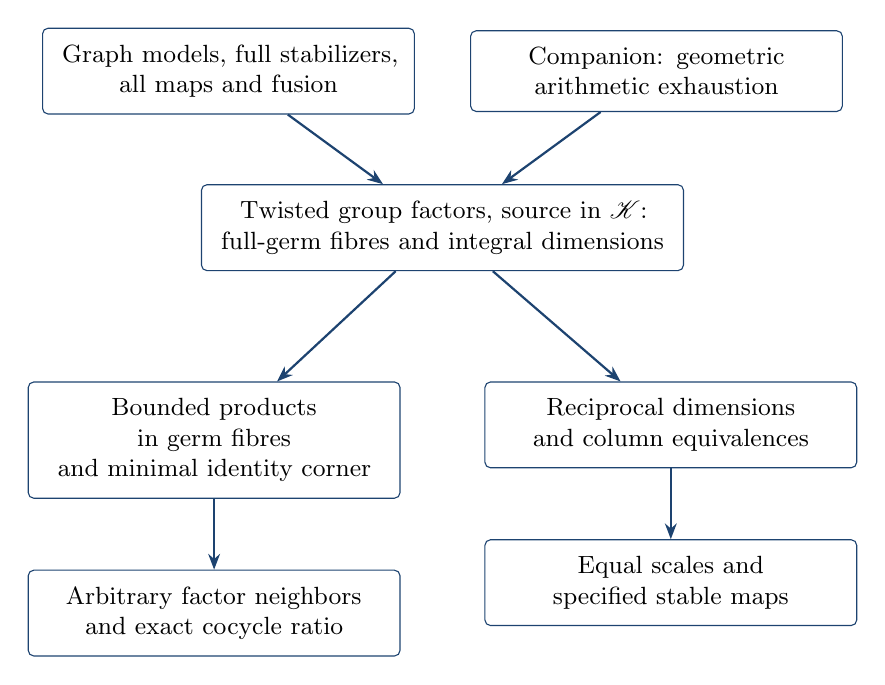
\begin{tikzpicture}[node distance=9mm and 7mm,
 box/.style={draw=linkblue,rounded corners=2pt,align=center,
 text width=43mm,inner sep=6pt,font=\small},
 arrow/.style={-{Stealth[length=2mm]},thick,draw=linkblue}]
\node[box] (models) {Graph models, full stabilizers,\\all maps and fusion};
\node[box,right=of models] (geometry) {Companion: geometric\\arithmetic exhaustion};
\node[box,below=of $(models.south)!0.5!(geometry.south)$,
 text width=57mm] (category) {Twisted group factors, source in $\mathscr K$:\\full-germ fibres and integral dimensions};
\node[box,below=14mm of category,xshift=-29mm] (mult) {Bounded products\\in germ fibres\\and minimal identity corner};
\node[box,below=14mm of category,xshift=29mm] (scale) {Reciprocal dimensions\\and column equivalences};
\node[box,below=of mult] (factor) {Arbitrary factor neighbors\\and exact cocycle ratio};
\node[box,below=of scale] (maps) {Equal scales and\\specified stable maps};
\draw[arrow] (models)--(category);
\draw[arrow] (geometry)--(category);
\draw[arrow] (category)--(mult);
\draw[arrow] (category)--(scale);
\draw[arrow] (mult)--(factor);
\draw[arrow] (scale)--(maps);
\end{tikzpicture}

\caption{Arithmetic exhaustion from the companion supplies the geometric input
for the main classification. The model calculus is independent of that input. Actual
multiplication and reciprocal dimensions are separate final arguments.}
\label{fig:proof-map}
\end{figure}

Section~\ref{sec:setup} records the relative tensor convention and exact
companion interface. Section~\ref{sec:calculus} proves all model formulas,
then applies exhaustion. Section~\ref{sec:endpoints} reconstructs factor
neighbors and specified stable maps. Section~\ref{sec:examples} proves the further consequences described above.

\section{Finite modules and the exhaustion interface}\label{sec:setup}

Our algebraic calculations need only countability and ICC. The geometric
class enters at one precise point: the exhaustion statement below says
that the explicit models contain every bifinite correspondence. We first
fix the norm convention for their construction.

For completeness, $L_\mu(\Gamma)$ is a factor when $\Gamma$ is ICC:
the absolute values of the Fourier coefficients of a central $L^2$ vector
are constant on conjugacy classes, so square summability kills every
nonidentity coefficient.

\subsection{Relative tensor products and elementary dimensions}
All Hilbert-space inner products are linear in the second variable.
A vector $\xi$ in an $M$--$N$ correspondence is \emph{right bounded}
if $R_\xi\widehat a=\xi a$ extends to a bounded map from $L^2(N)$.
For an $N$--$P$ correspondence, the relative tensor product is the
completion, after quotienting out zero-norm vectors, of the tensors
with right-bounded first vector and inner product
\begin{equation}\label{eq:relative-inner-product}
 \langle\xi\otimes_N\eta,\xi'\otimes_N\eta'\rangle
 =\langle\eta,(R_\xi^*R_{\xi'})\eta'\rangle.
\end{equation}
The right-module map $R_\xi^*R_{\xi'}$ is left multiplication by an
element of $N$. Balancing means
$(\xi a)\otimes_N\eta=\xi\otimes_N(a\eta)$ for $a\in N$.
This is the finite tracial form of Connes's relative tensor product
\cite[Chapter V, Appendix B, Theorems~13 and~20]{Connes1994}.

A finite right $N$-module has a column realization $pL^2(N)^n$,
with dimension $(\Tr_n\otimes\tau_N)(p)$. The vectors in $pN^n$
are right bounded and dense. The projection model and its dimension
are independent of the chosen realization
\cite[Theorem~10.1.1 and Proposition~10.1.3]{Jones2009}.
We prove the normality of the graph models directly in
Lemmas~\ref{lem:calculus-induction} and~\ref{lem:calculus-graph-model}.
The same elementary construction precedes the geometric argument in the
companion, so its exhaustion proof has no dependence on our all-maps or
summand classification. For $n=\dim\sigma$, the elementary dimensions are
$n[\Lambda:B]$ and $n[\Gamma:A]$ in left/right order. The dimensions of
\emph{actual summands} will require the full-stabilizer calculation.

\subsection{The geometric input}
The real simple factors in Definition~\ref{def:class} have higher rank
or are locally $\Sp(n,1)$, $n\geq2$, or $F_{4(-20)}$. At a finite
place their relative rank is at least two. Complex places are treated as
real Lie groups in differential arguments.
Property~$(T)$ passes between a locally compact group and a lattice and
between a discrete group and a finite-index subgroup; see \cite{BHV2008}. In particular,
that class is closed under abstract commensurability among countably
infinite ICC groups. The geometric companion treats arbitrary lattices
in the permitted finite products, without a dense-projection hypothesis.
We use exactly the following theorem.

\begin{proposition}[Arithmetic exhaustion, companion Theorem~1.2]
\label{prop:recovery-exhaustion}
Let $\Gamma\in\mathscr K$, let $\Lambda$ be any countably infinite ICC
group, and let $\mu,\omega$ be arbitrary normalized scalar cocycles.
Every nonzero separable bifinite
$L_\mu(\Gamma)$--$L_\omega(\Lambda)$ correspondence is a closed bimodule
summand of a finite direct sum of the models
$E(A,B,\delta,\sigma)$ in Equation~\eqref{eq:intro-model}, with the
exact multiplier in Equation~\eqref{eq:intro-multiplier}.
\end{proposition}

This is the Arithmetic exhaustion theorem of the complete companion
\cite[Theorem~1.2]{ArithmeticCompanion}. Its conclusion
retains actual finite-index subgroup isomorphisms and their exact scalar
ratios. We do not assume that the projective representations have finite
image, that either cocycle is finite type, or that the original
correspondence is irreducible. The algebraic proofs that follow are
independent of this proposition until its explicit application at the end
of Section~\ref{sec:calculus}.

\section{Full-germ correspondence calculus}\label{sec:calculus}

The calculations in this section are algebraic.  We give a group-factor
version of the projective induction and cocycle-corrected double-coset
calculus in Vaes's work on generalized Bernoulli crossed products
\cite[Theorem~2.2 and Section~6.2, especially Definition~6.8 and
Theorem~6.9]{Vaes2008}.  We prove the formulas here, including the
full-stabilizer argument for every bounded intertwiner and every bimodule
summand.  Until we apply
Proposition~\ref{prop:recovery-exhaustion}, the groups need only be countable
and ICC; the geometric hypotheses of Definition~\ref{def:class} are not
used.  We first construct the arithmetic models with their exact scalar
transports, and then determine their intertwiners, summands, conjugates,
and relative tensor products.  This order also verifies that every model
appearing in the exhaustion is a normal bifinite correspondence.

Write
\[
 M=L_\mu(\Gamma),\qquad N=L_\omega(\Lambda),\qquad
 D=\Gamma\times\Lambda,
 \qquad
 \alpha((g,h),(g',h'))=\mu(g,g')\overline{\omega(h,h')}.
\]
On an $M$--$N$ correspondence the joint group action is
\begin{equation}\label{eq:calculus-joint-action}
 U_{(g,h)}\xi=u_g\xi v_h^*.
\end{equation}
It has multiplier $\alpha$.  Indeed, its rightmost product is
$v_{h'}^*v_h^*=(v_hv_{h'})^*$, so
$U_{(g,h)}U_{(g',h')}=
\mu(g,g')\overline{\omega(h,h')}U_{(gg',hh')}$.
In particular the two coordinate actions commute exactly.

\subsection{Germs and their full stabilizers}

A germ from $\Gamma$ to $\Lambda$ is an isomorphism
$\delta:A\to B$ between finite-index subgroups, modulo agreement after
restriction to a common finite-index subgroup.  Composition means
composition on a finite-index domain where both representatives are
defined.  For example, if $\varepsilon:C\to F$ is a representative from
$\Lambda$ to a third group, then $\varepsilon\delta$ is defined on
$\delta^{-1}(B\cap C)$ and has image $\varepsilon(B\cap C)$.
Both have finite index in the relevant endpoint group.  Restricting
representatives further does not change the germ, and a common further
restriction verifies associativity.  Inversion is represented by the
inverse subgroup isomorphism.

For a germ $d$ from $\Gamma$ to $\Lambda$, let
\[
 (g,h)d=\Ad(h)\,d\,\Ad(g^{-1}),\qquad
 C_d=\{(g,h)\in D:(g,h)d=d\}.
\]
If $\delta:A\to B$ represents $d$, denote its graph by
$C_\delta=\{(a,\delta(a)):a\in A\}$.
We distinguish this graph from the full stabilizer $C_d$.

\begin{lemma}[Full stabilizers and the finite-orbit test]
\label{lem:calculus-germ-test}
The maps $g\mapsto[\Ad(g)]$ and $h\mapsto[\Ad(h)]$ are injective.
The group $C_d$ is the graph of an isomorphism
$\delta_d:A_d\to B_d$ between finite-index subgroups.  It contains
$C_\delta$ at finite index, and $\delta_d$ extends $\delta$.
If a finite-index subgroup of $C_d$ fixes another germ $x$ from
$\Gamma$ to $\Lambda$, then $x=d$.  Equivalently, the only finite
$C_d$-orbit in the space of these germs is $\{d\}$.
The same conclusion holds with $C_d$ replaced by $C_\delta$.
\end{lemma}

\begin{proof}
The centralizer of a finite-index subgroup of an ICC group is trivial:
an element of that centralizer has a centralizer of finite index and
therefore a finite conjugacy class.  This proves injectivity of the
inner-germ maps.

The stabilizer condition can be written
\begin{equation}\label{eq:calculus-stabilizer-relation}
 \Ad(h)=d\Ad(g)d^{-1}.
\end{equation}
If either coordinate of an element of $C_d$ is the identity, injectivity
of the inner-germ maps forces the other coordinate to be the identity.
Thus both coordinate projections on $C_d$ are injective.  Their images
$A_d$ and $B_d$ form the domain and range of a group isomorphism
$\delta_d$.  The inclusion $C_\delta\subset C_d$ follows by evaluating
Equation~\eqref{eq:calculus-stabilizer-relation} on a common finite-index
domain.  Consequently $A\subset A_d$, $B\subset B_d$, and
$\delta_d|_A=\delta$.  Both projected groups have finite index, and
$[C_d:C_\delta]=[A_d:A]<\infty$.

Suppose $C_0\leq C_d$ has finite index and fixes $x$.  Its first
projection $A_0$ has finite index in $\Gamma$.  For every
$(a,b)\in C_0$ the two stabilizer equations give
\begin{equation}\label{eq:calculus-finite-orbit-test}
 x\Ad(a)x^{-1}=\Ad(b)=d\Ad(a)d^{-1}.
\end{equation}
Choose representatives $\chi$ and $\delta$ for $x$ and $d$, and restrict
$a$ to $A_0\cap\operatorname{dom}(\chi)\cap
\operatorname{dom}(\delta)$.  On this finite-index subgroup the outer
expressions in Equation~\eqref{eq:calculus-finite-orbit-test} are the
inner germs of $\chi(a)$ and $\delta(a)$.  Injectivity in $\Lambda$
gives $\chi(a)=\delta(a)$, whence $x=d$.  A finite orbit has a
finite-index point stabilizer, so this proves the equivalent orbit
statement.  Finally, a finite-index subgroup of $C_\delta$ also has
finite index in $C_d$.
\end{proof}

The finite-orbit conclusion will make germ labels intrinsic to the
induced models.  Cosets of $C_d$ correspond to actual germs, whereas
several cosets of a presenting graph may represent the same germ.
After grouping those cosets, a bounded intertwiner will have matrix
blocks between the resulting finite-dimensional fibres.  Equivariance makes a block's
norm constant along a stabilizer orbit.  The lemma will therefore force
such a map to preserve each germ label, once square summability of its
columns is used.

\subsection{Projective induction and the arithmetic model}

Projective induction, induction in stages, and double-coset tensor
decompositions belong to Mackey's representation-theoretic framework
\cite[Theorems~4.1, 4.2, and~4.6]{Mackey1958}. The following coordinates fix the
multiplier throughout and prove every scalar identity used here.

Let $C\leq D$ be a subgroup and let $\gamma$ be a normalized unitary
projective representation on a finite-dimensional space $V$, with
multiplier $\alpha|_{C\times C}$.  Write $X=D/C$ for left cosets.
Choose representatives $r_x\in D$, with $r_C=e$, and give each $x\in X$
a copy $V_x$ of $V$.  Set
$\mathcal H(C,\gamma)=\bigoplus_{x\in X}V_x$, with the counting
Hilbert norm.  For $s\in D$ put
\begin{equation}\label{eq:input-A1}
 \begin{split}
 c(s,x)&=r_{sx}^{-1}sr_x,\\
 U^X_s(x)&=
 \frac{\alpha(s,r_x)}{\alpha(r_{sx},c(s,x))}\,
 \gamma(c(s,x)):V_x\longrightarrow V_{sx}.
 \end{split}
\end{equation}

\begin{lemma}[Exact projective induction]
\label{lem:calculus-induction}
Equation~\eqref{eq:input-A1} defines a unitary projective representation
of $D$ with multiplier $\alpha$.  Changing the coset representatives
gives a unitarily equivalent bundle by unitary identifications of its
individual fibres.  If $C$ is the graph of a finite-index subgroup
isomorphism $A\to B$, the bundle has commuting normal $M$ and right
$N$ actions, and is bifinite.
\end{lemma}

\begin{proof}
The correction $c(s,x)$ belongs to $C$, and
\[
 c(s,tx)c(t,x)=c(st,x).
\]
Using the cocycle identity for $\alpha$ and the projective multiplication
of $\gamma$ in Equation~\eqref{eq:input-A1} gives
\begin{equation}\label{eq:calculus-transport-identity}
 U^X_s(tx)U^X_t(x)=\alpha(s,t)U^X_{st}(x).
\end{equation}
One can also check all the scalar factors at once in the central
extension with multiplication
$(z,s)(w,t)=(zw\alpha(s,t),st)$: the representation of its preimage
of $C$ is $(z,c)\mapsto z\gamma(c)$, and the equality
$sr_x=r_{sx}c(s,x)$ gives exactly the ratio in
Equation~\eqref{eq:input-A1}.  Thus this argument retains, rather than
discards, the fixed multiplier.

For explicit independence of representatives, suppose
$r'_x=r_xk_x$, where $k_x\in C$.  The identification from the new
coordinate copy of $V_x$ to the old one is
\[
 F_x=\alpha(r_x,k_x)^{-1}\gamma(k_x).
\]
Indeed identifying a fibre by $U_{r'_x}$ instead of $U_{r_x}$ has
precisely this effect.  Equation~\eqref{eq:calculus-transport-identity}
then gives $F_{sx}U'{}^X_s(x)=U^X_s(x)F_x$.

Now assume that $C$ is a graph.  Both coordinate groups act freely on
$X$.  For example, if $(g,e)r_xC=r_xC$, then
$r_x^{-1}(g,e)r_x\in C$ has second coordinate $e$, so $g=e$.
On an orbit of the first coordinate group choose a fibre $V_{x_0}$.
The unitary identification
\[
 \ell^2(\Gamma)\otimes V_{x_0}\longrightarrow
 \bigoplus_{g\in\Gamma}V_{(g,e)x_0},
 \qquad \delta_g\otimes\xi\longmapsto U^X_{(g,e)}\xi
\]
intertwines its action with $\lambda_\mu\otimes1$, since
$U_{(a,e)}U_{(g,e)}=\mu(a,g)U_{(ag,e)}$.  Hence it extends normally
to $L_\mu(\Gamma)$.  The same argument for the second coordinate
gives copies of $\lambda_{\bar\omega}$, which are the standard
normal representations of the generators acting by right adjoints
$\xi\mapsto\xi v_h^*$.  The two actions commute, because the product
cocycle has trivial mixed-coordinate factors.

The first coordinate orbits are indexed by $\Lambda/B$, and the
second coordinate orbits by $\Gamma/A$.  They are finite in number.
Each is a regular module with multiplicity $\dim_{\mathbb C}V$,
proving bifiniteness as well as the dimension formulas below.
\end{proof}

We next identify this construction with the Connes-product model in
Theorem~\ref{thm:correspondences}.  This also supplies a direct normality
check of the subgroup action used to define that product.

\begin{lemma}[The graph-bundle unitary]
\label{lem:calculus-graph-model}
Let $\delta:A\to B$ be a finite-index subgroup isomorphism and let
$\sigma:A\to\mathcal U(V)$ have multiplier
$\beta=\mu|_{A\times A}/\delta^*\omega$.  Define
$\gamma(a,\delta(a))=\sigma(a)$.  Then
\[
 E(A,B,\delta,\sigma)=
 L^2(M)\mathbin{\bar\otimes}_{L_{\mu|A}(A)}
       (V\otimes L^2(N))
 \cong\mathcal H(C_\delta,\gamma).
\]
The unitary sends the vector $\xi$ in the fibre labelled by $x$ to
$U_{r_x}j\xi$, where
$j\xi=\widehat1\otimes(\xi\otimes\widehat1)$ in the displayed model.
\end{lemma}

\begin{proof}
On $V\otimes L^2(N)$ the subgroup action is
\[
 u_a(\xi\otimes\eta)=\sigma(a)\xi\otimes v_{\delta(a)}\eta.
\]
Its multiplier is $\beta(a,b)\omega(\delta(a),\delta(b))=\mu(a,b)$.
For normality, choose representatives $t$ for $B\backslash\Lambda$.
On the summand spanned by $\xi\otimes v_{\delta(a)}v_t$, the map
\begin{equation}\label{eq:calculus-absorption}
 \xi\otimes v_{\delta(a)}v_t
 \longmapsto\delta_a\otimes\sigma(a)^*\xi
 \quad\text{in }\ell^2(A)\otimes V
\end{equation}
is unitary and conjugates the subgroup action to
$\lambda_{\mu|A}\otimes1$.  To check the phase, applying $u_b$
before this map produces
\[
 \omega(\delta(b),\delta(a))
 \sigma(ba)^*\sigma(b)
 =\omega(\delta(b),\delta(a))\beta(b,a)\sigma(a)^*
 =\mu(b,a)\sigma(a)^*.
\]
Thus the left subgroup action is normal.  Its right $N$ action is
the standard action on the second factor and commutes with it.

Choose representatives $r$ for $\Gamma/A$.  As a right
$L_{\mu|A}(A)$ module, $L^2(M)$ has orthonormal free basis $u_r$;
the assertion follows directly from
$E_{L_{\mu|A}(A)}(u_r^*u_{r'})=\delta_{r,r'}1$.
The relative product therefore identifies with the orthogonal sum
\begin{equation}\label{eq:calculus-coset-model}
 E(A,B,\delta,\sigma)
 =\bigoplus_{r\in\Gamma/A}u_r\otimes(V\otimes L^2(N)).
\end{equation}
At its identity fibre the graph action is exactly
\[
 U_{(a,\delta(a))}j\xi
 =u_a\otimes(\xi\otimes v_{\delta(a)}^*)
 =j\sigma(a)\xi.
\]
For $g=ra$, balancing in Equation~\eqref{eq:calculus-coset-model}
gives the more explicit formula
\[
 U_{(g,h)}j\xi
 =\mu(r,a)^{-1}u_r\otimes
       \bigl(\sigma(a)\xi\otimes v_{\delta(a)}v_h^*\bigr).
\]
The last Fourier coordinate is $\delta(a)h^{-1}$, up to its displayed
unit scalar.  Thus two translated identity fibres are orthogonal
unless their labels in $D/C_\delta$ agree: equality of their first
cosets and last Fourier coordinates is exactly that coset equality.
Conversely these fibres exhaust every summand in
Equation~\eqref{eq:calculus-coset-model}.  They are an orthogonal,
transitive system with graph action $\gamma$ at the basepoint.
Finally
\[
 U_sU_{r_x}j
 =\frac{\alpha(s,r_x)}{\alpha(r_{sx},c(s,x))}
       U_{r_{sx}}j\gamma(c(s,x)),
\]
which proves that the stated unitary has exactly the transport
of Equation~\eqref{eq:input-A1}.
\end{proof}

For a full stabilizer we write
\[
 H(d,\gamma)=\mathcal H(C_d,\gamma).
\]
Its labels identify with actual germs in the orbit $Dd$.
There is also a canonical regrouping of an original graph model over
this full-germ orbit.  The map $D/C_\delta\to D/C_d$ has finite
fibres.  Its fibre above $C_d$ carries
\begin{equation}\label{eq:calculus-regrouping}
 \operatorname{Ind}^{C_d,\alpha}_{C_\delta}\gamma,
\end{equation}
where projective induction uses
Equation~\eqref{eq:input-A1} with $D$ replaced by $C_d$ and with the
restricted cocycle.  Indeed that fibre is the sum indexed by
$C_d/C_\delta$, and its transports are precisely that formula.
Regrouping the orthogonal sum consequently gives
\[
 \mathcal H(C_\delta,\gamma)
 \cong H\bigl(d,\operatorname{Ind}^{C_d,\alpha}_{C_\delta}\gamma\bigr).
\]
This description includes the phases of finite induction; it does not
replace the projective representation by an ordinary one.

Changing an orbit representative also retains a scalar transport.
If $d'=kd$, then $C_{d'}=kC_dk^{-1}$.  Identify the new base fibre
with the old one using $U_k$.  For $c'=kck^{-1}\in C_{d'}$ the
representation in these coordinates is
\begin{equation}\label{eq:calculus-representative-change}
 \gamma'(c')=
 \frac{\alpha(c',k)}{\alpha(k,c)}\,\gamma(c).
\end{equation}
Indeed $U_{c'}U_k=
\alpha(c',k)\alpha(k,c)^{-1}U_kU_c$.
This gives the exact representative-change equivalence, including its
restricted multiplier.  Two choices of $k$ leading to the same germ
give equivalent fibres by the stabilizer action itself.

\begin{proposition}[Dimensions of the actual orbit modules]
\label{prop:calculus-dimensions}
For a finite-dimensional $\alpha|_{C_d}$-projective representation
$\gamma$,
\begin{equation}\label{eq:calculus-full-dimensions}
 \dim_M H(d,\gamma)
   =\dim_{\mathbb C}(\gamma)[\Lambda:B_d],
 \qquad
 \dim H(d,\gamma)_N
   =\dim_{\mathbb C}(\gamma)[\Gamma:A_d].
\end{equation}
For the original model these formulas read
\[
 \dim_M E(A,B,\delta,\sigma)
   =\dim_{\mathbb C}(\sigma)[\Lambda:B],
 \qquad
 \dim E(A,B,\delta,\sigma)_N
   =\dim_{\mathbb C}(\sigma)[\Gamma:A].
\]
Zero fibres may be omitted.  Dimensions add under finite orthogonal
sums.
\end{proposition}

\begin{proof}
The free coordinate-orbit identifications in
Lemma~\ref{lem:calculus-induction} exhibit exactly the stated numbers
of copies of the standard left and right modules.  Each standard
module has dimension one for the normalized factor trace.
Lemma~\ref{lem:calculus-graph-model} gives the original-model formulas.
\end{proof}

\subsection{All bounded intertwiners and all summands}

\begin{theorem}[Full-germ intertwiner formula]
\label{thm:calculus-hom}
Choose finitely many distinct $D$-orbits of germs and a representative
$d$ in each orbit.  Let $\gamma_d,\tau_d$ be finite-dimensional
projective representations of $C_d$, with multiplier $\alpha|_{C_d}$;
either may be zero.  Then
\begin{equation}\label{eq:calculus-hom}
 \Hom_{M\text{--}N}
 \left(\bigoplus_dH(d,\gamma_d),\,
       \bigoplus_dH(d,\tau_d)\right)
 =\bigoplus_d\Hom_{C_d,\alpha}(\gamma_d,\tau_d).
\end{equation}
The equality is implemented by restriction to the representative
fibres and extension by transport.  Norm is the maximum of the fibre
norms, and adjoints and composition are fibrewise.  In particular all
closed bimodule summands are obtained by taking invariant subspaces
of these finite-dimensional fibre representations.
\end{theorem}

\begin{proof}
Realize both modules over their union of full-germ orbits, assigning a
zero fibre where necessary.  An intertwiner $T$ has finite-dimensional
matrix blocks $T_{yx}:V_x\to W_y$.  If $(e_i)$ is an orthonormal basis
of $V_x$, then
\begin{equation}\label{eq:calculus-hs-column}
 \sum_y\|T_{yx}\|_{\mathrm{HS}}^2
 =\sum_i\|Te_i\|^2
 \leq\dim(V_x)\|T\|^2<\infty.
\end{equation}
Equivariance identifies $T_{sy,sx}$ with
$U^\tau_s(y)T_{yx}U^\gamma_s(x)^*$.  Its Hilbert--Schmidt norm is
therefore unchanged.  For $s\in C_x$, Equation~\eqref{eq:calculus-hs-column}
implies that a nonzero block $T_{yx}$ can occur only when the
$C_x$-orbit of $y$ is finite.  By
Lemma~\ref{lem:calculus-germ-test}, this forces $y=x$.
Thus every intertwiner is diagonal in the germ labels, including
between initially different orbit bundles.

At a representative label $d$, equivariance is exactly the requirement
that $T_d$ intertwine the two $\alpha|_{C_d}$-projective
representations.  Conversely, such an operator extends by
\[
 T_{sd}=U^\tau_s(d)T_dU^\gamma_s(d)^*.
\]
This is independent of the choice of $s$: changing $s$ by an element
of $C_d$ uses the intertwining identity, and the identical scalar
multiplier on both sides cancels.  The extension is bounded with norm
$\|T_d\|$ on that orbit and commutes with every joint group generator.
Normality of the endpoint representations then makes it a bimodule
intertwiner.  This proves Equation~\eqref{eq:calculus-hom} and the
norm assertion.  The formulas for adjoint and composition follow
on each fibre.

A closed bimodule summand is the range of a projection in the bounded
bimodule commutant.  The preceding description identifies that
projection with a family of $C_d$-equivariant fibre projections.
Their ranges are precisely the asserted projective-representation
summands, and their transported ranges give the entire module summand.
\end{proof}

Consider any closed bimodule summand $K$ of a finite sum of the original
graph models. Regroup each model by Equation~\eqref{eq:calculus-regrouping},
combine copies of the same full-germ orbit, and apply
Theorem~\ref{thm:calculus-hom} to the projection onto $K$.  We obtain a finite
orthogonal sum of full-germ bundles, with exactly the intertwiners
in Equation~\eqref{eq:calculus-hom}.  In particular, if its fibre
representations are $\rho_d$, its actual dimensions are
\begin{equation}\label{eq:calculus-summand-dimensions}
 \dim_M K=\sum_d\dim_{\mathbb C}(\rho_d)[\Lambda:B_d],
 \qquad
 \dim K_N=\sum_d\dim_{\mathbb C}(\rho_d)[\Gamma:A_d].
\end{equation}
Both are positive integers for $K\ne0$.  This conclusion uses the
description of its projection; the dimensions of a containing model
alone would not imply it.

\begin{remark}[Why a presenting graph must be enlarged]
Let $M=N=L_\mu(\Gamma)$, with arbitrary $\mu$, and suppose
$A<\Gamma$ has finite index $k>1$.  Present the identity germ $d$
by $\id_A:A\to A$, with the one-dimensional trivial fibre.
The multiplier on every diagonal pair is
$\mu(a,b)\overline{\mu(a,b)}=1$, so this is a model for any source
twist.  Its full stabilizer is the diagonal copy of $\Gamma$.
Regrouping therefore replaces the presenting fibre by the permutation
representation on $\ell^2(\Gamma/A)$.

The constant vectors form an invariant line.  Its orthogonal projection
has every matrix entry equal to $1/k$, and selects
$H(d,1)=L^2(M)$ from the model $E(A,A,\id_A,1)$.
The selected module has dimensions $(1,1)$, whereas the containing model
has dimensions $(k,k)$.  On each of the $k$ original one-dimensional
fibres above $d$, the diagonal block of the selecting projection is $1/k$, which
is not a projection.  Grouping those fibres at the full stabilizer is
what exposes the invariant line and its actual rank.
\end{remark}

\subsection{Conjugation}

On the conjugate correspondence $\overline{\mathcal H(C,\gamma)}$
the endpoint groups are swapped.  Its subgroup and base fibre are
\[
 C^{\mathrm{op}}=\{(h,g):(g,h)\in C\},\qquad
 \bar\gamma(h,g)\bar\xi=\overline{\gamma(g,h)\xi}.
\]
The multiplier is
$\omega\boxtimes\bar\mu$, since
$\bar\gamma$ conjugates $\alpha$ and swaps its two variables.
The label $x$ of a full-germ bundle becomes the inverse germ $x^{-1}$:
indeed
\[
 \bigl(\Ad(h)x\Ad(g^{-1})\bigr)^{-1}
 =\Ad(g)x^{-1}\Ad(h^{-1}).
\]
With swapped coset representatives, the transport is explicitly
\begin{equation}\label{eq:calculus-conjugate-transport}
 U^{\bar X}_{(h,g)}(\bar x)
   =\overline{U^X_{(g,h)}(x)}.
\end{equation}
Thus it includes the conjugate of the scalar ratio in
Equation~\eqref{eq:input-A1}.  At the module level this equality is
the defining identity
$v_h\bar\xi u_g^*=\overline{u_g\xi v_h^*}$.
For an original graph $\delta:A\to B$, the new graph is
$\delta^{-1}:B\to A$ and its fibre representation is
$b\mapsto\overline{\sigma(\delta^{-1}(b))}$.
Fibre intertwiners are conjugated by the same rule; their adjoints and
norms are preserved.  Proposition~\ref{prop:calculus-dimensions}
also shows directly that the left and right dimensions are exchanged.

\subsection{Balanced fusion and its scalar transport}

Let $P=L_\nu(\Pi)$.  Consider a bundle $\mathcal H_X$ from
$(\Gamma,\mu)$ to $(\Lambda,\omega)$ and a bundle $\mathcal H_Y$
from $(\Lambda,\omega)$ to $(\Pi,\nu)$, each constructed as above.
Write $V_x$ and $W_y$ for their fibres and
$\alpha'=\omega\boxtimes\bar\nu$.  Finite direct sums are handled
by distribution, so we may first take one transitive bundle at each
endpoint.  Define
\begin{equation}\label{eq:calculus-balanced-labels}
 Z=(X\times Y)/\Lambda,
 \qquad h(x,y)=\bigl((1,h)x,(h,1)y\bigr).
\end{equation}
Identify the tensor fibres along this action using
\begin{equation}\label{eq:calculus-middle-transport}
 J_h(x,y)=U^X_{(1,h)}(x)\otimes U^Y_{(h,1)}(y).
\end{equation}
These identifications are genuine unitary group transports, because
their multiplier is
$\overline{\omega(h_1,h_2)}\omega(h_1,h_2)=1$.
The action on labels is free, as already its action on $X$ is free.
Each quotient fibre $V_z$ is consequently unambiguously a tensor
fibre after choosing one representative of $z$.  Put
$\mathcal H_Z=\bigoplus_{z\in Z}V_z$, with counting norm at any
such representatives.  Changing representatives gives a unitary
identification by Equation~\eqref{eq:calculus-middle-transport}.

The outer transport before passage to the quotient is
$U^X_{(g,1)}\otimes U^Y_{(1,k)}$.  It commutes exactly with every
$J_h$: each mixed-coordinate factor of either product cocycle is
one.  Its multiplier is $\mu\boxtimes\bar\nu$.
For an explicit formula choose a representative $(x,y)$ of $z$ and
representatives for all quotient labels.  There is a unique $h$ such
that
\[
 \bigl((g,h)x,(h,k)y\bigr)
\]
is the chosen representative of $(g,k)z$.  With
$s=(g,h)$, $t=(h,k)$, $c=c_X(s,x)$ and $b=c_Y(t,y)$, the quotient
transport is
\begin{equation}\label{eq:input-A2}
 \frac{\alpha(s,r_x)\alpha'(t,r_y)}
      {\alpha(r_{sx},c)\alpha'(r_{ty},b)}
       \gamma_X(c)\otimes\gamma_Y(b).
\end{equation}
It is the product of the two transports in
Equation~\eqref{eq:input-A1}.  There is no additional factor from
the compensating element $h$, since its lift is the genuine
transport in Equation~\eqref{eq:calculus-middle-transport}.

To attach a germ to a quotient label, first recall the map from graph
cosets to germs.  For $x=(g,h)C_\delta\in X$, put
\[
 d_x=\Ad(h)[\delta]\Ad(g^{-1}),
\]
and define $d_y$ in the same way for $y\in Y$.  These are the
graph-coset-to-germ maps from the earlier regrouping, applied at their
respective endpoints; they need not be injective.  The middle action changes the two associated germs by
\[
 (d_x,d_y)\longmapsto
       (\Ad(h)d_x,\,d_y\Ad(h^{-1})).
\]
Hence $z=[(x,y)]\mapsto d_y d_x$ is well defined.  Distinct quotient
labels can still have the same germ; the next proposition explains how
their fibres are regrouped.

\begin{proposition}[Fusion as a counting tensor-fibre bundle]
\label{prop:calculus-fusion}
There is a unitary correspondence identification
\begin{equation}\label{eq:calculus-fusion-unitary}
 \mathcal H_X\mathbin{\bar\otimes}_{N}\mathcal H_Y
 \cong\mathcal H_Z
\end{equation}
under which outer transport is Equation~\eqref{eq:input-A2}.
The space $Z$ has finitely many outer-group orbits.  For each
$z=[(x,y)]$, its stabilizer is a finite-index subgroup-isomorphism
graph with germ $d_y d_x$.
Regrouping these orbits over full stabilizers by
Equation~\eqref{eq:calculus-regrouping} gives the full-germ
decomposition of the fusion.
\end{proposition}

\begin{proof}
First we check the Hilbert norm and the relative product explicitly.
Every $\xi\in V_x$ is right bounded: the map
\[
 R_\xi:L^2(N)\longrightarrow\mathcal H_X,
 \qquad \widehat n\longmapsto\xi n
\]
initially defined on the group algebra extends with norm $\|\xi\|$.
Indeed the vectors $\xi v_h$ occupy distinct fibres as $h$ varies,
and all have norm $\|\xi\|$.  Choose one $x_i$ in each right
$\Lambda$-orbit of $X$, and an orthonormal basis $(e_{ij})_j$ of
$V_{x_i}$.  Orthogonality of all their group translates gives
\[
 R_{e_{ij}}^*R_{e_{i'j'}}=\delta_{ii'}\delta_{jj'}1.
\]
Their ranges exhaust $\mathcal H_X$, because the translates exhaust
every labelled fibre.  They therefore form an orthonormal free
right $N$ basis, with finitely many elements.

The defining inner product of the relative tensor product now gives
\begin{equation}\label{eq:calculus-relative-inner-product}
 \left\langle e_{ij}\otimes_N\eta,
                 e_{i'j'}\otimes_N\eta'\right\rangle
 =\delta_{ii'}\delta_{jj'}\langle\eta,\eta'\rangle.
\end{equation}
Thus that product is unitarily
$\bigoplus_i(V_{x_i}\otimes\mathcal H_Y)$.
Every label in $Z$ has a unique representative with first coordinate
one of the fixed $x_i$: freeness of the right action on $X$ gives
uniqueness of the required balancing element.  Consequently the
counting tensor-fibre Hilbert sum $\mathcal H_Z$ is exactly this
same orthogonal sum.  Its map to the relative product sends
$\xi\otimes\eta\in V_x\otimes W_y$ to
$\xi\otimes_N\eta$.  Equation~\eqref{eq:calculus-relative-inner-product}
proves that it is isometric and onto.  It is independent of the
representative, since
\begin{equation}\label{eq:calculus-balanced-vector}
 (\xi v_h^*)\otimes_N(v_h\eta)
 =\xi\otimes_N(v_h^*v_h\eta)
 =\xi\otimes_N\eta.
\end{equation}
Applying the outer generators to these vectors proves
Equation~\eqref{eq:input-A2} at the correspondence level.

For finiteness and the stabilizers we give the explicit double-coset
calculation, which also specifies the composed germ and its fibre
representation.  Write the two graph maps as
\[
 \delta:A\longrightarrow B\leq\Lambda,
 \qquad \varepsilon:C\longrightarrow F\leq\Pi,
\]
with $A\leq\Gamma$ and $C\leq\Lambda$ of finite index, and
take $X=(\Gamma\times\Lambda)/C_\delta$,
$Y=(\Lambda\times\Pi)/C_\varepsilon$.
Choose $m$ in the finite double-coset set $B\backslash\Lambda/C$.
Represent its outer orbit by
\[
 z_m=[(C_\delta,(m,1)C_\varepsilon)].
\]
Outer translation and balancing send an arbitrary pair to the form
\[
 ((g,h)C_\delta,(\ell,k)C_\varepsilon)
 \longmapsto(C_\delta,(h^{-1}\ell,1)C_\varepsilon).
\]
Changing the initial coset representatives replaces $h^{-1}\ell$
by $\delta(a)^{-1}h^{-1}\ell c$ for $a\in A$, $c\in C$.
Hence these outer orbits are indexed exactly by
$B\backslash\Lambda/C$.

An outer element $(a,p)$ stabilizes $z_m$ precisely when some $h$
satisfies
\[
 (a,h)\in C_\delta,
 \qquad (m^{-1}hm,p)\in C_\varepsilon.
\]
Its stabilizer is consequently the graph of
\begin{equation}\label{eq:calculus-composed-graph}
 \begin{split}
 A_m&=\delta^{-1}(B\cap mCm^{-1}),\\
 \theta_m&=\varepsilon\circ\Ad(m^{-1})\circ\delta:A_m\longrightarrow F_m,\\
 F_m&=\varepsilon(C\cap m^{-1}Bm).
 \end{split}
\end{equation}
Both projections have finite index.  In particular
\begin{equation}\label{eq:calculus-double-coset-labels}
 Z\cong\bigsqcup_{m\in B\backslash\Lambda/C}
             (\Gamma\times\Pi)/C_{\theta_m}.
\end{equation}
Here $C_{\theta_m}$ denotes the graph of the displayed actual map,
not necessarily its full-germ stabilizer.
At $z_m$ the composite germ is
$[\varepsilon\Ad(m^{-1})\delta]=[\theta_m]$.
Its graph lies at finite index in its full stabilizer by
Lemma~\ref{lem:calculus-germ-test}.  This proves all the stated
regrouping assertions.
\end{proof}

For completeness, the last proof yields an explicit finite
double-coset formula without unspecified stabilizer representations.
Let $\sigma$ and $\tau$ be the original fibre representations on
$A$ and $C$.  In the fibre at $z_m$ choose $r_{(m,1)C_\varepsilon}=(m,1)$.
For $a\in A_m$, write $b=\delta(a)$ and $c=m^{-1}bm\in C$.
Equation~\eqref{eq:input-A2}, with compensating element $h=b$, gives
\begin{equation}\label{eq:calculus-double-coset-fibre}
 \gamma_m(a)=
 q_m(b)\,\sigma(a)\otimes\tau(m^{-1}bm),
 \qquad
 q_m(b)=\frac{\omega(b,m)}{\omega(m,m^{-1}bm)}.
\end{equation}
The correction has the exact coboundary
\begin{equation}\label{eq:calculus-conjugation-coboundary}
 \frac{q_m(b)q_m(b')}{q_m(bb')}
 =\frac{\omega(b,b')}
 {\omega(m^{-1}bm,m^{-1}b'm)}.
\end{equation}
To verify this, the twisted group-unit identity
$v_bv_m=q_m(b)v_mv_{m^{-1}bm}$ can be multiplied successively for
$b,b'$ and compared with the identity for $bb'$.
Combining Equation~\eqref{eq:calculus-conjugation-coboundary} with
the multipliers of $\sigma$ and $\tau$ shows that $\gamma_m$ has
multiplier $\mu|_{A_m}/\theta_m^*\nu$.  Hence
\begin{equation}\label{eq:calculus-double-coset-fusion}
 E(A,B,\delta,\sigma)\mathbin{\bar\otimes}_N
 E(C,F,\varepsilon,\tau)
 \cong\bigoplus_{m\in B\backslash\Lambda/C}
      E(A_m,F_m,\theta_m,\gamma_m).
\end{equation}
The appropriate endpoint algebras in the second model and in each
summand are understood from their displayed groups.
One then applies finite projective induction to the full stabilizers
and combines any equal full-germ orbits.  Formula
\eqref{eq:calculus-double-coset-fibre} exhibits explicitly why replacing
the twisted fusion rule by its ordinary version would lose a phase.

The indices in Equation~\eqref{eq:calculus-composed-graph} satisfy
\[
 [\Gamma:A_m]=[\Gamma:A][B:B\cap mCm^{-1}],
 \qquad
 [\Pi:F_m]=[\Pi:F][C:C\cap m^{-1}Bm].
\]
Counting the left $B$-orbits in $\Lambda/C$ and the right $C$-orbits
in $B\backslash\Lambda$ gives, respectively,
\[
 \sum_m[B:B\cap mCm^{-1}]=[\Lambda:C],
 \qquad
 \sum_m[C:C\cap m^{-1}Bm]=[\Lambda:B].
\]
Thus both coordinate groups have finitely many orbits in the fused
label space.  These formulas also verify, directly from the models
and their counting norms, the usual multiplicativity of the left
dimensions and of the right dimensions under this fusion.

\subsection{Maps, associativity, and completion of the calculus}

The preceding identifications respect the entire operator calculus,
not only the isomorphism classes of objects.  For the map calculation,
first regroup the inputs into full-germ bundles.
Theorem~\ref{thm:calculus-hom} then represents every bounded intertwiner
by an equivariant family of fibre maps.  An equivariant family
$T_x:V_x\to V'_x$ and an equivariant family $S_y:W_y\to W'_y$
give the fibre maps $T_x\otimes S_y$.  They commute with the
middle identifications in Equation~\eqref{eq:calculus-middle-transport},
so descend to the quotient fibres.  Under the unitary of
Proposition~\ref{prop:calculus-fusion}, they are precisely
$T\mathbin{\bar\otimes}_N S$, as is seen on
$\xi\otimes_N\eta$.  Their norms are bounded by $\|T\|\|S\|$;
adjoints and compositions agree fibrewise.  Regrouping by finite
projective induction is a regrouping of these same Hilbert fibres
and maps.  Conjugation has the map formula already given in
Equation~\eqref{eq:calculus-conjugate-transport}.

For three bundles, both orders of fusion use the quotient of the
triple label space by the two middle groups.  Their actions commute:
on the shared middle bundle they are its commuting coordinate
actions, and their projective factors cancel with those in the
adjacent bundles.  The fibre identification between the two orders
is the ordinary unitary
\[
 (\xi\otimes\eta)\otimes\zeta
       \longmapsto\xi\otimes(\eta\otimes\zeta).
\]
The counting norms and Equation~\eqref{eq:calculus-relative-inner-product}
show that it is also the canonical associativity unitary for the
relative products.  All scalar identifications are those of
Equation~\eqref{eq:calculus-middle-transport}; hence this assertion
requires no change of cocycle.  For any further number of factors
these maps agree on elementary tensors, which are total, so the
associativity identifications are coherent.  The unit correspondence
$L^2(M)$ is the identity-germ model with its one-dimensional trivial
graph representation; its unit maps are ordinary left and right
multiplication on the corresponding relative tensors.

Conjugation reverses a balanced product.  The unitary
\[
 \overline{\mathcal H_X\mathbin{\bar\otimes}_N\mathcal H_Y}
 \longrightarrow
 \overline{\mathcal H_Y}\mathbin{\bar\otimes}_N
       \overline{\mathcal H_X},
 \qquad
 \overline{\xi\otimes_N\eta}
       \longmapsto\bar\eta\otimes_N\bar\xi
\]
is well defined on tensors of vectors in labelled fibres: the
simultaneous middle transport
becomes the same transport on the swapped conjugate fibres, with
both scalar factors conjugated and their product still one.
The counting tensor-fibre model of
Proposition~\ref{prop:calculus-fusion} proves preservation of the norm:
the map bijects the quotient labels and is unitary on each conjugate
tensor fibre.  These tensors are total.  It intertwines the swapped
endpoint actions and the conjugated fibre maps.  Thus the conjugation,
unit, and associativity identifications agree with those of the
correspondence category at the level of actual operators.

We now apply the geometric input. Proposition~\ref{prop:recovery-exhaustion}
places every bifinite correspondence with source in $\mathscr K$ inside
a finite sum of graph models. The preceding full-germ calculation resolves
its selecting projection into fibre projections. Together with the operation
formulas just proved, this establishes every assertion of
Theorem~\ref{thm:correspondences}, including
all bounded intertwiners, actual summands and their dimensions, and
the specified conjugation and fusion maps.  Throughout the section
only the matched-subgroup ratio is required to have a
finite-dimensional projective realization.  None of the calculations
imposes a finite-image condition on that representation or a
finite-type condition on either individual endpoint cocycle.

\section{Arbitrary factor endpoints and stable canonical recovery}
\label{sec:endpoints}

We now use the correspondence classification to recover the multiplication
of an unknown factor.  The argument first realizes that factor, up to
amplification, as a finite-index extension of the given twisted group
factor.  Its self-correspondence grading then consists of bounded
operators and respects the actual product.  This additional multiplication
step is what turns the correspondence data into a group presentation.
The homogeneous-product and minimal-corner construction has a direct
predecessor in Donvil--Vaes \cite[Proposition~6.5 and Theorem~6.6]{DonvilVaes2025}.
Their construction already permits arbitrary source cocycles and recovers
the exact matched ratio. We adapt it from globally defined automorphism
degrees to finite-index isomorphism germs.

\subsection{A finite-index extension and its intrinsic grading}

\begin{lemma}[From a bifinite neighbor to an extension]
\label{lem:endpoints-extension}
Let \(M,P\) be \(\mathrm{II}_1\) factors and let \({}_M K_P\ne0\) be
bifinite.  The commutant \(Q\) of the right \(P\)-action is a positive
finite amplification of \(P\), and the given left action identifies
\(M\) with a unital finite-index subfactor of \(Q\).
\end{lemma}

\begin{proof}
The finite right module has a column realization
\(K=pL^2(P)^n\), with
\(r=(\Tr_n\otimes\tau_P)(p)=\dim K_P>0\).
Its right-action commutant is
\(Q=p(M_n(\mathbb C)\bar\otimes P)p=P^r\), equipped with the
normalized corner trace.  The left action of \(M\) is a normal unital
embedding into \(Q\), because a nonzero representation of a factor has
zero kernel.  Its restriction preserves normalized trace.

As a left \(Q\)-module, \(K\) has finite positive dimension \(1/r\).
Choose an integer \(j\) with \(j/r\geq1\).  Comparison of finite
module projections embeds \(L^2(Q)\) as a left \(Q\)-submodule of
\(K^{\oplus j}\).  Restriction to \(M\) makes it a finite left
\(M\)-module.  Thus the Jones index \([Q:M]=\dim_M L^2(Q)\) is
finite.  This uses the standard finite-factor column and index
identifications; see \cite{Jones1983} and \cite[Theorem~10.1.1, Proposition~10.1.3, and Theorem~10.2.1]{Jones2009}.
\end{proof}

Fix \(\Gamma\in\mathscr K\), an arbitrary normalized scalar cocycle
\(\mu\), and \(M=L_\mu(\Gamma)\).  Write
\(D=\Comm(\Gamma)\) for the group of virtual automorphism germs
defined in Section~\ref{sec:calculus}. The map
\[
 \iota:\Gamma\longrightarrow D,\qquad
 \iota(g)=[\Ad(g)],
\]
is injective: an element in its kernel centralizes a finite-index
subgroup of \(\Gamma\), and hence has a finite conjugacy class.
For a representative \(\delta:A\to B\) of \(d\in D\), one has
\begin{equation}
 d\,\iota(a)\,d^{-1}=\iota(\delta(a))\qquad(a\in A).
 \label{eq:endpoints-inner-germs}
\end{equation}

\begin{lemma}[The intrinsic self-correspondence grading]
\label{lem:endpoints-grading}
Every bifinite \(M\)--\(M\) correspondence has an orthogonal decomposition
\[
 K=\bigoplus_{d\in D}K_d
\]
into finite-dimensional spaces, with only countably many nonzero terms,
such that
\[
 u_gK_du_h^*=K_{\iota(g)d\iota(h)^{-1}}.
\]
The support is contained in finitely many \(\iota(\Gamma)\)-double
cosets.  For every representative \(\delta:A\to B\) of \(d\),
\begin{equation}
 K_d=\left\{\xi\in K:
  \dim_{\mathbb C}\operatorname{span}
    \{u_{\delta(a)}\xi u_a^*:a\in A\}<\infty\right\}.
 \label{eq:input-B1}
\end{equation}
In particular, for the fixed presentation $M=L_\mu(\Gamma)$, the
grading is determined by the two actions and does not depend on a
choice of arithmetic model decomposition.
\end{lemma}

\begin{proof}
Apply Theorem~\ref{thm:correspondences} and the full-germ decomposition
of Section~\ref{sec:calculus}.  Use the inverse of its germ labels, so
that our degree is a germ from the right group to the left group.
If \(x\) is an old label and \(d=x^{-1}\), the old action gives
\[
 \bigl(\Ad(h)x\Ad(g^{-1})\bigr)^{-1}
 =\iota(g)d\iota(h)^{-1}.
\]
Combining the finitely many representation fibres at each identical
inverse label gives \(K_d\) and the stated covariance. The finitely
many old germ orbits become finitely many
\(\iota(\Gamma)\)-double cosets. Separability makes the nonzero
support countable.

For a representative \(\delta\), the operators
\(U_a\xi=u_{\delta(a)}\xi u_a^*\) preserve \(K_d\).
Their multiplier is
\(\mu(\delta(a),\delta(b))\overline{\mu(a,b)}\).
They form a projective unitary representation, so its orbit span is
invariant, even when the multiplier is not trivial.  This proves the
forward inclusion in Equation~\eqref{eq:input-B1}.

Conversely let \(W\) be a finite-dimensional invariant orbit span and
choose an orthonormal basis \(\xi_1,\ldots,\xi_l\) of \(W\).
If \(P_x\) projects onto \(K_x\), the numbers
\[
 m(x)=\sum_{i=1}^l\|P_x\xi_i\|^2
\]
have finite sum \(l\) and are invariant under
\(x\mapsto\iota(\delta(a))x\iota(a)^{-1}\).
Indeed \(U_a\) permutes the degree spaces and carries the chosen basis
of \(W\) to another orthonormal basis.  Positive mass is therefore
possible only on a finite orbit.  The stabilizer of such an \(x\)
contains a finite-index subgroup \(A_0\leq A\), and
\[
 x\iota(a)x^{-1}=\iota(\delta(a))\qquad(a\in A_0).
\]
Represent \(x\) by \(\epsilon:C\to E\) and restrict to
\(A_0\cap C\).  Equation~\eqref{eq:endpoints-inner-germs} and
injectivity of \(\iota\) give \(\epsilon(a)=\delta(a)\) there.
Thus \(x=d\).  All of \(W\) lies in \(K_d\), proving the converse
and the asserted intrinsic description.
\end{proof}

\subsection{Bounded homogeneous operators and the minimal corner}

Let \(M\subset Q\) now be a unital finite-index inclusion of
\(\mathrm{II}_1\) factors and apply Lemma~\ref{lem:endpoints-grading}
to \({}_M L^2(Q)_M\).  Until the next lemma, its degree spaces are only
Hilbert subspaces of \(L^2(Q)\).

\begin{lemma}[Boundedness and multiplication]
\label{lem:endpoints-bounded-grades}
Every \(K_d\) consists of bounded elements of \(Q\), and
\begin{equation}
 K_dK_f\subset K_{df},\qquad K_d^*=K_{d^{-1}},\qquad
 1\in K_1,\qquad u_a\in K_{\iota(a)}.
 \label{eq:endpoints-grade-product}
\end{equation}
Consequently \(K_1\) is a finite-dimensional unital \(*\)-subalgebra
of \(Q\), normalized by the \(u_a\), and \(\tau_Q(K_d)=0\) for
\(d\ne1\).
\end{lemma}

\begin{proof}
Let $\xi\in K_d$. For distinct $g\in\Gamma$, the right translates
$\xi u_g$ have distinct degrees $d\iota(g)$. Injectivity of $\iota$
therefore gives $\langle\xi,\xi u_g\rangle=0$ for $g\ne e$.
Initially put $a=\xi^*\xi\in L^1(Q)_+$. The $L^1$ extension of the
trace expectation satisfies
\[
 E_M(a)=\|\xi\|_2^2 1:
\]
indeed, for each $g\in\Gamma$,
\[
 \tau_M(E_M(a)u_g)=\tau_Q(a u_g)=\langle\xi,\xi u_g\rangle.
\]
These values agree with those of $\|\xi\|_2^2 1$. They determine
the normal functional associated to $E_M(a)\in L^1(M)$, because the
group algebra is ultraweakly dense in $M$. For the bounded spectral
truncations $a_n=\min(a,n)$,
Pimsner--Popa's finite-index inequality
\cite[Proposition~2.1]{PimsnerPopa1986} gives
\[
 [Q:M]^{-1}a_n\leq E_M(a_n)\leq E_M(a)=\|\xi\|_2^2 1.
\]
Monotone convergence makes $a$ bounded, and hence $\xi\in Q$, with
$\|\xi\|_\infty\leq[Q:M]^{1/2}\|\xi\|_2$. This argument uses
orthogonality of the degrees, so the scalar phases in the right action
do not change it. We now verify the product itself.

Take \(\xi\in K_d\), \(\eta\in K_f\), and representatives
\(\delta:A\to B\), \(\epsilon:C\to E\).  On the finite-index
domain \(C_0=\{a\in C:\epsilon(a)\in A\}\), the exact identity
\[
 u_{\delta\epsilon(a)}\xi\eta u_a^*
   =(u_{\delta\epsilon(a)}\xi u_{\epsilon(a)}^*)
      (u_{\epsilon(a)}\eta u_a^*)
\]
puts the orbit of the product into the finite-dimensional span of
products of bases of \(K_d\) and \(K_f\).
These are bounded elements, as just proved.  The intrinsic test
\eqref{eq:input-B1} yields \(\xi\eta\in K_{df}\).
Taking adjoints in the same test gives
\(K_d^*\subset K_{d^{-1}}\), and taking adjoints again gives equality.
The vector \(1\) is fixed by the identity graph.  For the graph of
\(\Ad(a)\), the vector \(u_a\) is carried to a scalar multiple of
itself, since the corresponding product of group labels is \(a\).
Thus its graph orbit span is one-dimensional, even with the twist.
This proves Equation~\eqref{eq:endpoints-grade-product}.

Finite dimension of \(K_1\) comes from the grading lemma, and
normalization follows from its covariance.  Orthogonality to
\(1\in K_1\) gives the trace assertion for other degrees.
\end{proof}

Compressing $K_1$ to a scalar algebra will now force each surviving
degree to be a unitary line.

\begin{lemma}[The minimal identity corner]
\label{lem:endpoints-minimal-corner}
Let \(p\) be a minimal projection of \(K_1\).  There are a countable
subgroup \(\Lambda\leq D\) and a normalized scalar cocycle \(\omega\)
such that the actual corner \(pQp\), with normalized trace, is
isomorphic to \(L_\omega(\Lambda)\).  Each nonzero space \(pK_dp\)
is one-dimensional and has a unitary basis vector in the corner.
\end{lemma}

\begin{proof}
Left and right multiplication by \(p\) are commuting orthogonal
projections on \(L^2(Q)\).  They preserve each degree by
Equation~\eqref{eq:endpoints-grade-product}; their product projects
onto \(L^2(pQp)\).  Thus, up to the common normalization factor of
the corner trace,
\[
 L^2(pQp)=\bigoplus_{d\in D}pK_dp,\qquad pK_1p=\mathbb Cp.
\]
For \(0\ne x\in pK_dp\), the product and adjoint laws give
\(x^*x=\alpha p\) and \(xx^*=\beta p\), with positive scalars.
Traciality gives \(\alpha=\beta\).  Therefore
\(x/\sqrt\alpha\) is a unitary in \(pQp\).
If \(y\) belongs to the same degree, \(x^*y\in\mathbb Cp\), so
\(y\) is a scalar multiple of \(x\).

Set \(\Lambda=\{d:pK_dp\ne0\}\).  It contains the identity, is
closed under inverses, and is closed under products because products
of its homogeneous unitaries cannot vanish.  It is countable by
orthogonality and separability.  Choose unitary vectors
\(v_d\in pK_dp\), with \(v_1=p\), and define
\[
 v_dv_f=\omega(d,f)v_{df}.
\]
Unitarity makes the coefficient unimodular, associativity gives the
2-cocycle identity, and \(v_1=p\) gives normalization.
The \(v_d\) form an orthonormal basis for the normalized corner
trace.  The unitary \(\delta_d\mapsto v_d\) from \(\ell^2(\Lambda)\)
to \(L^2(pQp)\) intertwines twisted left regular multiplication with
left multiplication by these units.

Let \(Q_0\) be the von Neumann algebra they generate.  The
trace-preserving expectation onto \(Q_0\) has \(L^2\)-range containing
every \(v_d\), so it has full range and \(Q_0=pQp\).
The basis unitary therefore gives a normal unital complex-linear
\(*\)-isomorphism \(L_\omega(\Lambda)\cong pQp\), as claimed.
\end{proof}

\subsection{The ratio condition and the reconstructed group}

The minimal corner has supplied a twisted group algebra, but the group
$\Lambda$ still needs to satisfy the hypotheses of
Theorem~\ref{thm:endpoints}. We next recover a finite-index copy of a
subgroup of $\Gamma$ inside $\Lambda$, obtain the projective ratio from
the identity matrix block, and prove that $\Lambda$ is ICC.

\begin{proposition}[Arithmetic constraints on the corner]
\label{prop:endpoints-corner-constraints}
For the corner in Lemma~\ref{lem:endpoints-minimal-corner}, the group
\(\Lambda\) is countably infinite and ICC.  There are finite-index
subgroups \(A\leq\Gamma\), \(B\leq\Lambda\), an actual group
isomorphism \(\delta:A\to B\), and a finite-dimensional projective
representation with multiplier
\(\mu|_A/\delta^*(\omega|_B)\).
\end{proposition}

\begin{proof}
Let \(z\) be the central support of \(p\) in the finite-dimensional
algebra \(K_1\), so that \(zK_1\) is the matrix block containing
\(p\). We first split the action on this block from the homogeneous
unitaries that will survive in \(pQp\).
The subgroup
\[
 A=\{a\in\Gamma:u_azu_a^*=z\}
\]
has finite index, because conjugation permutes the finitely many
central blocks. Although these conjugations preserve $z$, they may move
$p$ inside its matrix block. We therefore remove their action on that
block before compressing. Choose unitary matrix implementers
\(s_a\in\mathcal U(zK_1)\), \(s_e=z\), for
\(\Ad(u_a)|_{zK_1}\).  Since these automorphisms form an ordinary
group action, there is a normalized scalar cocycle \(\kappa\) with
\[
 s_as_b=\kappa(a,b)s_{ab}.
\]
These matrices already constitute a finite-dimensional projective
representation.  Their image is allowed to be infinite.

The unitaries \(q_a=s_a^*u_az\in zQz\) commute with \(zK_1\).
Using \(u_as_b^*u_a^*=s_as_b^*s_a^*\), their product is
\begin{align*}
 q_aq_b
  &=s_a^*(u_as_b^*u_a^*)u_au_bz\\
  &=\mu(a,b)s_b^*s_a^*u_{ab}z
    =\mu(a,b)\overline{\kappa(a,b)}q_{ab}.
\end{align*}
They are homogeneous of degree \(\iota(a)\), and they commute with
\(p\).  Their compressions \(t_a=pq_ap\) are therefore corner
unitaries in \(pK_{\iota(a)}p\), satisfying the same product formula.
It follows that \(B=\iota(A)\) lies in \(\Lambda\), and that
\(\delta=\iota|_A:A\to B\) is an actual isomorphism.

To compare their multiplier with the cocycle already chosen in
Lemma~\ref{lem:endpoints-minimal-corner}, write the basis unitary of
degree \(\iota(a)\) as
\(v_{\iota(a)}=\lambda(a)t_a\), where $\lambda:A\to\mathbb T$
and $\lambda(e)=1$. With the convention
\[
 (\partial\lambda)(a,b)=\lambda(a)\lambda(b)\lambda(ab)^{-1},
\]
we obtain
\begin{equation}
 \delta^*\omega=(\partial\lambda)\mu|_A\,\overline\kappa,
 \qquad
 \frac{\mu|_A}{\delta^*\omega}
       =(\partial\lambda)^{-1}\kappa.
 \label{eq:endpoints-ratio}
\end{equation}
On the defining space of the block, the matrices
\(a\mapsto\overline{\lambda(a)}s_a\) realize precisely the
second multiplier.  This is the required ratio condition.

We have the subgroup isomorphism and its exact ratio. It remains to
show that its image has finite index in \(\Lambda\) and that
\(\Lambda\) is ICC. Put \(H=\iota(\Gamma)\).
Every \(d\in D\) commensurates \(H\), by
Equation~\eqref{eq:endpoints-inner-germs} on a finite-index domain.
Consequently each double coset \(HdH\) is a finite union of right
\(H\)-cosets.  Lemma~\ref{lem:endpoints-grading} puts the original
degree support in finitely many such double cosets.  Since \(B\) has
finite index in \(H\), that support is contained in finitely many
right \(B\)-cosets.  The subgroup \(\Lambda\) is contained in this
support and contains \(B\); hence \([\Lambda:B]<\infty\).
In particular it is infinite.

Suppose \(l\in\Lambda\) has finite conjugacy class. Its centralizer
$C_\Lambda(l)$ has finite index in \(\Lambda\). Thus
$A_0=\iota^{-1}(C_\Lambda(l)\cap B)$ has finite index in
$\Gamma$, and $l$ centralizes \(\iota(A_0)\).
Represent its germ by \(\epsilon:C\to E\).  For
\(a\in A_0\cap C\), centralization and
Equation~\eqref{eq:endpoints-inner-germs} give
\(\iota(\epsilon(a))=\iota(a)\).
Injectivity of \(\iota\) gives \(\epsilon(a)=a\) on this
finite-index subgroup.  Thus \(l=1\) in \(D\), proving ICC.
The construction uses only subgroup isomorphisms and introduces no
finite kernel.
\end{proof}

\begin{proof}[Proof of Theorem~\ref{thm:endpoints}]
Apply Lemma~\ref{lem:endpoints-extension} to the given nonzero bifinite
correspondence. It gives a finite-index extension
\(M\subset Q=P^r\).  The preceding lemmas and
Proposition~\ref{prop:endpoints-corner-constraints} give
\(pQp\cong L_\omega(\Lambda)\) with the asserted group and ratio
data.  Since \(pQp\) is the amplification
\(P^{r\tau_Q(p)}\), standard column equivalences give
\[
 P\cong L_\omega(\Lambda)^t,
 \qquad t=(r\tau_Q(p))^{-1}>0.
\]

Conversely the stated subgroup and projective data give a nonzero
bifinite arithmetic correspondence from \(M\) to
\(L_\omega(\Lambda)\), by Section~\ref{sec:calculus}.
Compose it with the corner equivalence from that factor to its
amplification and then with the specified factor isomorphism to \(P\).
This is a nonzero bifinite \(M\)--\(P\) correspondence.

When \(\mu=1\), conjugating the finite-dimensional ratio
representation and transporting it through \(\delta\) gives a
representation with multiplier \(\omega|_B\).  Projective induction
from \(B\) to \(\Lambda\), with the given global multiplier
\(\omega\), is finite-dimensional and realizes \(\omega\) itself;
compare \cite[Lemmas~6.7--6.8]{DonvilVaes2025}. The induction formula of Section~\ref{sec:calculus} applies equally to
this finite-index subgroup.  For general \(\mu\) the construction
proves only the exact ratio in Equation~\eqref{eq:endpoints-ratio},
as required.
\end{proof}

\subsection{Stable scales and the actual isomorphism}

For a specified stable isomorphism, the category gives a different
constraint: its equivalence correspondence has reciprocal dimensions.
After integrality forces both dimensions to be one, we will use the
given corner columns to identify the specified map. All dimensions below
use the normalized factor traces and the ordinary unnormalized matrix
trace $\Tr_n$, with $\Tr_n(1)=n$.

\begin{lemma}[Dimension and corner equivalences]
\label{lem:endpoints-equivalence-dimensions}
For composable bifinite correspondences of finite factors, left
dimensions multiply under relative tensor product, and so do right
dimensions.  If
\(M^t=p(M_n(\mathbb C)\bar\otimes M)p\) and
\(C_p=pL^2(M)^n\), then \({}_{M^t}C_p{}_M\) is an equivalence
correspondence with dimensions \((1/t,t)\) in left/right order.
\end{lemma}

\begin{proof}
For the right-dimension assertion, realize a right \(N\)-module
\(H\) as \(eL^2(N)^k\).  Then
\(H\otimes_N K=eK^k\).  The normalized trace on the finite factor
\(\operatorname{End}(K_P)\) restricts to the normalized trace on its
unital copy of \(N\).  Computing the dimension of \(eK^k\) therefore
gives
\[
 \dim(H\otimes_N K)_P
  =(\Tr_k\otimes\tau_N)(e)\,\dim K_P.
\]
The left formula follows by conjugating the correspondences.
The column \(C_p\) has right dimension \(t\) by its defining
projection.  The standard column pairings identify
\(C_p\otimes_M\overline{C_p}\) with \(L^2(M^t)\) and
\(\overline{C_p}\otimes_{M^t}C_p\) with \(L^2(M)\).
The multiplication formula makes its left dimension \(1/t\).
These identifications use the normalized corner trace, which accounts
for the reciprocal scale.
\end{proof}

\begin{proof}[Proof of Theorem~\ref{thm:stable}]
Set \(M=L_\omega(\Lambda)\) and \(N=L_\nu(\Pi)\).
Use the actual given corner presentations
\[
 M^t=pM_n(M)p,\qquad N^s=qM_m(N)q,
\]
and the columns \(C_p=pL^2(M)^n\), \(C_q=qL^2(N)^m\).
A specified isomorphism \(\theta:M^t\to N^s\) gives the
\(M\)--\(N\) equivalence correspondence
\begin{equation}
 H_\theta=\overline{C_p}\otimes_{M^t}
 {}_\theta L^2(N^s)\otimes_{N^s}C_q.
 \label{eq:endpoints-lifted-isomorphism}
\end{equation}
By Lemma~\ref{lem:endpoints-equivalence-dimensions}, its left and right
dimensions are \(t/s\) and \(s/t\). Theorem~\ref{thm:correspondences}
applies to \(H_\theta\) because \(\Lambda\in\mathscr K\) and
\(\Pi\) is countably infinite ICC. Its full-germ decomposition and
Equation~\eqref{eq:calculus-summand-dimensions} make both numbers
positive integers. Their product is one, so \(t=s\).

The same formula now forces a single full-germ orbit, a
one-dimensional fibre, and both stabilizer projections equal to the
whole endpoint groups.  Indeed each nonzero orbit contributes its
positive integer fibre dimension times a positive integer subgroup
index to each of the two sums, both of which equal one.  Thus its
graph is an actual group isomorphism \(\delta:\Lambda\to\Pi\).
Consequently \(\Pi\in\mathscr K\), since \(\Lambda\in\mathscr K\)
and this class is invariant under group isomorphism.
The one-dimensional fibre is a normalized cochain \(b:\Lambda\to
\mathbb T\) with
\[
 \omega(g,h)=b(g)b(h)b(gh)^{-1}\nu(\delta(g),\delta(h)).
\]
The arithmetic bundle identification in Section~\ref{sec:calculus}
therefore gives
\(H_\theta\cong {}_\varphi L^2(N)\), where
\[
 \varphi(u_g)=b(g)v_{\delta(g)}.
\]
Multiplication and the displayed cochain equation define a
\(*\)-homomorphism on the group algebra.  Its trace-preserving basis
unitary extends it to a normal unital isomorphism \(M\to N\).

We now return to the specified map in its actual corners. First choose
any partial isometry between the corresponding projections; then the
correspondence identification will supply the inner correction that makes
it implement \(\theta\). The projections
\(\varphi^{(n)}(p)\) and \(q\) have equal unnormalized trace \(t=s\).
Comparison of projections in the finite matrix amplification of
\(N\) gives a rectangular partial isometry
\[
 z\in M_{m,n}(N),\qquad
 z^*z=\varphi^{(n)}(p),\qquad zz^*=q.
\]
Define
\(\theta_0(x)=z\varphi^{(n)}(x)z^*\) on \(pM_n(M)p\).
Its lifted correspondence in
Equation~\eqref{eq:endpoints-lifted-isomorphism} is
\({}_\varphi L^2(N)\).  To check this directly, on bounded columns
set $F(\xi)=z\varphi^{(n)}(\xi)$, applying $\varphi$ entrywise.
For $x\in pM_n(M)p$, $a\in M$, and $\xi,\eta\in pM^{n}$, one has
\[
 F(x\xi a)=\theta_0(x)F(\xi)\varphi(a),\qquad
 F(\xi)^*F(\eta)=\varphi(\xi^*\eta).
\]
Moreover $F$ is onto the bounded columns $qN^m$, since $zz^*=q$.
These identities, followed by the normalized column pairings of
Lemma~\ref{lem:endpoints-equivalence-dimensions}, contract the two
column factors to the trace module with left action \(\varphi\).

Consequently \(H_\theta\cong H_{\theta_0}\).  Tensor on the left
with \(C_p\) and on the right with \(\overline{C_q}\); the column
equivalences cancel and give a unitary
\[
 U:{}_\theta L^2(N^s)\longrightarrow {}_{\theta_0}L^2(N^s).
\]
A right-linear unitary on this standard trace module is left
multiplication by a unitary \(w\in N^s\).
Its left intertwining identity says
\(w\theta(x)=\theta_0(x)w\).
Replacing \(z\) by \(w^*z\), which has the same initial and final
projections, therefore yields the actual formula
\begin{equation}
 \theta(x)=z\varphi^{(n)}(x)z^*
 \qquad(x\in pM_n(M)p).
 \label{eq:endpoints-actual-corner-map}
\end{equation}
At ordinary unit scale this is precisely
\(\theta(u_g)=z\,b(g)v_{\delta(g)}z^*\) with \(z\in N\) unitary.

Conversely a group isomorphism and normalized cochain satisfying the
cocycle equation construct \(\varphi\) by the same basis unitary.
At equal scales, comparison of the two actual projections supplies
\(z\), and Equation~\eqref{eq:endpoints-actual-corner-map} constructs
the corner isomorphism.  This proves both directions and the
specified-map assertion.  Taking identical factor inputs and scales
\(1,t\) shows that every factor in the statement has fundamental
group \(\{1\}\).
\end{proof}

\section{Commensurability, named lattices, and endomorphisms}
\label{sec:examples}

The category calculation gives concise consequences with different
mathematical content. Untwisted correspondence existence detects abstract
commensurability. Stable isomorphism recovers an entire group and a
specified map. A finite-index endomorphism requires one additional
classical covolume argument; its two module dimensions are not initially
reciprocal.

\subsection{Untwisted correspondences and finite-type neighbors}

\begin{corollary}\label{cor:commensurability}
Let $\Gamma\in\mathscr K$ and let $\Lambda$ be any countably infinite
ICC group. There is a nonzero bifinite $L(\Gamma)$--$L(\Lambda)$
correspondence if and only if $\Gamma$ and $\Lambda$ are abstractly
commensurable.
\end{corollary}
\begin{proof}
A nonzero correspondence has a nonzero full-germ orbit in
Theorem~\ref{thm:correspondences}. Its stabilizer is the graph of an
actual isomorphism between finite-index subgroups. Conversely such an
isomorphism, with its one-dimensional trivial fibre representation,
gives the model in Equation~\eqref{eq:intro-model}.
\end{proof}

With the finite-type convention of Section~\ref{sec:introduction},
the endpoint theorem specializes as follows.
\begin{corollary}\label{cor:untwisted-neighbors}
For $\Gamma\in\mathscr K$, a separable $\mathrm{II}_1$ factor $P$ is
joined to $L(\Gamma)$ by a nonzero bifinite correspondence if and only if
$P\cong L_\omega(\Lambda)^t$ for $t>0$, an ICC group $\Lambda$
abstractly commensurable with $\Gamma$, and a finite-type cocycle
$\omega$ on $\Lambda$.
\end{corollary}
\begin{proof}
Theorem~\ref{thm:endpoints} and the final projective-induction argument
in its proof give necessity. For sufficiency, restrict a projective
representation of multiplier $\omega$ to the matched subgroup and
conjugate it; its multiplier is exactly $1/\delta^*\omega$. The graph
model and the amplification equivalence give the required correspondence.
\end{proof}

For arbitrary source twist this specialization must be replaced by the
ratio in Theorem~\ref{thm:endpoints}. In particular, its direct proof
admits the identity correspondence of $L_\mu(\Gamma)$ whatever the
individual cocycle $\mu$ may be.

\subsection{Examples and specified canonical maps}

The familiar arithmetic examples are
$\mathrm{SL}_3(\mathbb Z)$, its principal congruence subgroup
\[
 \Gamma(3)=\ker\bigl(\mathrm{SL}_3(\mathbb Z)
                    \longrightarrow\mathrm{SL}_3(\mathbb Z/3\mathbb Z)\bigr),
\]
all their finite-index subgroups, $\mathrm{PSL}_n(\mathbb Z)$ for
$n\geq4$, and $\mathrm{PSp}_4(\mathbb Z)$, with the latter two
symbols denoting the quotient by the center of the integral matrix
group. The arithmetic lattice theorem places these projective groups in
the corresponding center-free real groups \cite{BorelHarishChandra1962}; the finite-covolume statement appears also in
\cite[Theorem~1(iv)]{BorelHarishChandra1961}.
For even $n$, $\mathrm{PSL}_n(\mathbb R)$ is the identity root-generated
subgroup of $\mathrm{PGL}_n(\mathbb R)$; for odd $n$ it is all of it.
Likewise $\mathrm{PSp}_4(\mathbb R)$ is the root-generated adjoint
symplectic group. These ambient groups have real rank at least two and
property~$(T)$ \cite{BHV2008}.

These projective lattices are ICC. A finite conjugacy class gives a
finite-index centralizer. That subgroup is Zariski dense by Borel density,
so the element centralizes the connected ambient algebraic group and is
trivial in its adjoint form \cite{Borel1960}. Equivalently, the centralizer formulation in
\cite[Corollary~3]{Furstenberg1976} applies directly to the finite-index
lattice and gives the ambient center. For
$\mathrm{SL}_3(\mathbb Z)$ the real center is already trivial.
A finite-index subgroup of an ICC group remains ICC: its finite
conjugacy class would yield a finite class in the ambient group after
using finitely many coset representatives. Thus every group just listed
belongs to $\mathscr K$.

For any such group $\Gamma$, any countably infinite ICC group $\Lambda$,
and any specified isomorphism
\[
 \theta:L(\Gamma)\longrightarrow pM_k(L(\Lambda))p,
\]
Theorem~\ref{thm:stable} yields
\[
 (\Tr_k\otimes\tau)(p)=1,\qquad
 \theta(u_g)=\chi(g)Wv_{\delta(g)}W^*,\qquad
 W^*W=1,\quad WW^*=p,
\]
where $W\in M_{k,1}(L(\Lambda))$,
$\delta:\Gamma\to\Lambda$ is an actual group isomorphism, and
$\chi:\Gamma\to\mathbb T$ is a character. This includes the
specified column in the specified corner. The character becomes the
cochain of Equation~\eqref{eq:intro-cochain} when scalar twists are
present. In particular all the corresponding twisted factors have
fundamental group $\{1\}$.

Definition~\ref{def:class} also includes ICC lattices in the permitted
finite-place groups, mixed real and finite-place products, and products
with quaternionic or Cayley real factors of property~$(T)$. Finite
products of the preceding discrete examples give reducible cases:
a nonidentity element has a nonidentity coordinate with infinite
conjugacy class. More generally the companion exhaustion theorem already
allows arbitrary reducible lattices, nonuniform lattices, and torsion.
No repetition of the individual geometric proofs is required for these
examples.

\begin{corollary}[Outer automorphisms]\label{cor:outer-automorphisms}
For $\Gamma\in\mathscr K$, there is an isomorphism of abstract groups
\[
 \operatorname{Out}(L(\Gamma))
 \cong\Hom(\Gamma,\mathbb T)\rtimes\operatorname{Out}(\Gamma),
 \qquad [\delta]\cdot\chi=\chi\circ\delta^{-1},
\]
where $\operatorname{Out}$ denotes automorphisms modulo inner
automorphisms.
\end{corollary}
\begin{proof}
Put $T_\chi(u_g)=\chi(g)u_g$ and $U_\delta(u_g)=u_{\delta(g)}$.
These maps extend normally by their trace-preserving basis unitaries.
Characters are invariant under inner group automorphisms, and
$U_\delta T_\psi U_\delta^{-1}=T_{\psi\circ\delta^{-1}}$.
Thus $(\chi,[\delta])\mapsto[T_\chi U_\delta]$ is a well-defined
homomorphism for the displayed left action. It is surjective by the
untwisted unit-scale case of Theorem~\ref{thm:stable}, whose cochain
is then a character.

For injectivity, suppose $T_\chi U_\delta=\Ad(w)$, and write
$b=\chi\circ\delta$ and $w=\sum_x a_xu_x$ in $L^2(L(\Gamma))$.
The relation
\[
 u_{\delta(g)}wu_g^{-1}=b(g)^{-1}w
\]
shows that $|a_x|$ is constant on each orbit of
$x\mapsto\delta(g)xg^{-1}$. A nonzero coefficient has a finite orbit
by square summability. Its stabilizer $H$ has finite index, and
$\delta(h)=xhx^{-1}$ for all $h\in H$.
Set $\beta=\Ad(x^{-1})\circ\delta$ and let $N$ be the normal core
of $H$. Since $\beta$ fixes $N$ pointwise,
$g^{-1}\beta(g)$ centralizes $N$ for every $g\in\Gamma$.
The centralizer of a finite-index subgroup is trivial by ICC, as in
Lemma~\ref{lem:calculus-germ-test}; hence $\delta=\Ad(x)$.
Now $v=u_x^*w$ implements the pure character twist $b$.
Its Fourier-coefficient absolute values are constant on conjugacy
classes, so ICC makes $v$ scalar. Therefore $b=1$, whence $\chi=1$,
and $[\delta]=1$, proving injectivity.
\end{proof}

\subsection{Recovery from the reduced group C*-algebra}

Write $C_r^*(\Gamma)$ for the operator-norm closure of the group algebra
in the left regular representation.
\begin{corollary}[Reduced C*-algebra recovery]\label{cor:reduced-cstar}
Let $\Gamma\in\mathscr K$ and suppose that $C_r^*(\Gamma)$ has a
unique tracial state. If $\Lambda$ is any discrete group and
there is a complex-linear $*$-isomorphism
$C_r^*(\Gamma)\cong C_r^*(\Lambda)$, then
$\Gamma\cong\Lambda$.
\end{corollary}
\begin{proof}
Let $\alpha:C_r^*(\Gamma)\to C_r^*(\Lambda)$ be the given
$*$-isomorphism, and denote the canonical traces by $\tau_\Gamma$
and $\tau_\Lambda$. The isomorphism is unital, and uniqueness gives
$\tau_\Lambda\circ\alpha=\tau_\Gamma$. Consequently $\alpha$
extends isometrically to a unitary between the trace-GNS Hilbert
spaces. This unitary intertwines left multiplication, so conjugation by
it extends $\alpha$ to a normal isomorphism
$L(\Gamma)\cong L(\Lambda)$.

The source reduced algebra is separable. Distinct canonical group
unitaries in the target have trace $2$-norm distance $\sqrt2$, and hence
operator-norm distance at least $\sqrt2$; thus $\Lambda$ is countable.
Moreover, $L(\Lambda)$ is an infinite-dimensional factor, so $\Lambda$
is infinite and ICC. Indeed, a nonidentity finite conjugacy class would
give a nonscalar central class sum. Theorem~\ref{thm:stable}, with both
cocycles trivial and both amplification scales equal to one, now gives
$\Gamma\cong\Lambda$.
\end{proof}

In particular this applies to $\Gamma=\mathrm{SL}_3(\mathbb Z)$:
its reduced group C*-algebra has a unique tracial state by
\cite[discussion following Corollary~5]{Bekka2007}.

\subsection{Finite-index endomorphisms of the special linear factor}

We state the precise classical fact needed in the final deduction.
The finite-index image hypothesis is part of it.
\begin{lemma}\label{lem:sl3-covolume}
An injective homomorphism
$\alpha:\mathrm{SL}_3(\mathbb Z)\to\mathrm{SL}_3(\mathbb Z)$
whose image has finite index is surjective.
\end{lemma}
\begin{proof}
Put $G=\mathrm{SL}_3(\mathbb R)$ and $\Gamma=\mathrm{SL}_3(\mathbb Z)$.
The group $G$ is connected, center-free, simple, of real rank two, and
has no compact factor. Both $\Gamma$ and $\alpha(\Gamma)$ are
irreducible lattices in $G$. The classical strong-rigidity theorem
extends their isomorphism to an analytic automorphism $\Phi$ of $G$;
see \cite[Theorem~B]{Prasad1973}. This form of strong rigidity allows
nonuniform lattices and torsion; its excluded real rank-one
$\mathrm{SL}_2(\mathbb R)$ case does not occur here. The theorem
combines the uniform rigidity of Mostow with the nonuniform higher-rank
work of Margulis and Raghunathan and Prasad's extension, as explained
in that reference.

The differential $D=d\Phi_e$ preserves the nondegenerate Killing form
$B$ on the Lie algebra: $D^{\mathsf T}BD=B$. Hence $|\det D|=1$.
A left-invariant Haar density is therefore preserved at the identity
and, by translation, everywhere. Consequently
\[
 \operatorname{covol}(\alpha(\Gamma))
 =\operatorname{covol}(\Phi(\Gamma))
 =\operatorname{covol}(\Gamma).
\]
On the other hand the first covolume equals
$[\Gamma:\alpha(\Gamma)]\operatorname{covol}(\Gamma)$.
The common covolume is positive and finite, so the index equals one.
\end{proof}

\begin{corollary}\label{cor:sl3-endomorphism}
Every normal unital complex-linear $*$-endomorphism $\theta$ of
$M=L(\mathrm{SL}_3(\mathbb Z))$ with $[M:\theta(M)]<\infty$
is surjective.
\end{corollary}
\begin{proof}
The endomorphism is injective because its kernel is an ultraweakly
closed two-sided ideal in a factor, and it preserves the normalized trace. Equip $H=L^2(M)$ with its usual
right action and the left action $x\xi=\theta(x)\xi$. It is bifinite,
with
\[
 \dim H_M=1,\qquad \dim_M H=[M:\theta(M)].
\]
Its actual full-germ decomposition and
Equation~\eqref{eq:calculus-summand-dimensions} show that right dimension
one leaves exactly one orbit, a one-dimensional fibre, and
$A_d=\mathrm{SL}_3(\mathbb Z)$. The graph is therefore an isomorphism
$\delta:\mathrm{SL}_3(\mathbb Z)\to B_d$, where $B_d$ has finite
index in the same group. Lemma~\ref{lem:sl3-covolume} makes $B_d$ the
whole group. The left dimension formula now gives $[M:\theta(M)]=1$,
so $\theta(M)=M$.
\end{proof}

\bibliographystyle{amsplain}
\bibliography{references}
\end{document}
